% Options for packages loaded elsewhere
\PassOptionsToPackage{unicode}{hyperref}
\PassOptionsToPackage{hyphens}{url}
%
\documentclass[
]{book}
\usepackage{lmodern}
\usepackage{amssymb,amsmath}
\usepackage{ifxetex,ifluatex}
\ifnum 0\ifxetex 1\fi\ifluatex 1\fi=0 % if pdftex
  \usepackage[T1]{fontenc}
  \usepackage[utf8]{inputenc}
  \usepackage{textcomp} % provide euro and other symbols
\else % if luatex or xetex
  \usepackage{unicode-math}
  \defaultfontfeatures{Scale=MatchLowercase}
  \defaultfontfeatures[\rmfamily]{Ligatures=TeX,Scale=1}
\fi
% Use upquote if available, for straight quotes in verbatim environments
\IfFileExists{upquote.sty}{\usepackage{upquote}}{}
\IfFileExists{microtype.sty}{% use microtype if available
  \usepackage[]{microtype}
  \UseMicrotypeSet[protrusion]{basicmath} % disable protrusion for tt fonts
}{}
\makeatletter
\@ifundefined{KOMAClassName}{% if non-KOMA class
  \IfFileExists{parskip.sty}{%
    \usepackage{parskip}
  }{% else
    \setlength{\parindent}{0pt}
    \setlength{\parskip}{6pt plus 2pt minus 1pt}}
}{% if KOMA class
  \KOMAoptions{parskip=half}}
\makeatother
\usepackage{xcolor}
\IfFileExists{xurl.sty}{\usepackage{xurl}}{} % add URL line breaks if available
\IfFileExists{bookmark.sty}{\usepackage{bookmark}}{\usepackage{hyperref}}
\hypersetup{
  pdftitle={Introdução ao R com aplicações em biodiversidade e conservação},
  hidelinks,
  pdfcreator={LaTeX via pandoc}}
\urlstyle{same} % disable monospaced font for URLs
\usepackage{color}
\usepackage{fancyvrb}
\newcommand{\VerbBar}{|}
\newcommand{\VERB}{\Verb[commandchars=\\\{\}]}
\DefineVerbatimEnvironment{Highlighting}{Verbatim}{commandchars=\\\{\}}
% Add ',fontsize=\small' for more characters per line
\usepackage{framed}
\definecolor{shadecolor}{RGB}{248,248,248}
\newenvironment{Shaded}{\begin{snugshade}}{\end{snugshade}}
\newcommand{\AlertTok}[1]{\textcolor[rgb]{0.94,0.16,0.16}{#1}}
\newcommand{\AnnotationTok}[1]{\textcolor[rgb]{0.56,0.35,0.01}{\textbf{\textit{#1}}}}
\newcommand{\AttributeTok}[1]{\textcolor[rgb]{0.77,0.63,0.00}{#1}}
\newcommand{\BaseNTok}[1]{\textcolor[rgb]{0.00,0.00,0.81}{#1}}
\newcommand{\BuiltInTok}[1]{#1}
\newcommand{\CharTok}[1]{\textcolor[rgb]{0.31,0.60,0.02}{#1}}
\newcommand{\CommentTok}[1]{\textcolor[rgb]{0.56,0.35,0.01}{\textit{#1}}}
\newcommand{\CommentVarTok}[1]{\textcolor[rgb]{0.56,0.35,0.01}{\textbf{\textit{#1}}}}
\newcommand{\ConstantTok}[1]{\textcolor[rgb]{0.00,0.00,0.00}{#1}}
\newcommand{\ControlFlowTok}[1]{\textcolor[rgb]{0.13,0.29,0.53}{\textbf{#1}}}
\newcommand{\DataTypeTok}[1]{\textcolor[rgb]{0.13,0.29,0.53}{#1}}
\newcommand{\DecValTok}[1]{\textcolor[rgb]{0.00,0.00,0.81}{#1}}
\newcommand{\DocumentationTok}[1]{\textcolor[rgb]{0.56,0.35,0.01}{\textbf{\textit{#1}}}}
\newcommand{\ErrorTok}[1]{\textcolor[rgb]{0.64,0.00,0.00}{\textbf{#1}}}
\newcommand{\ExtensionTok}[1]{#1}
\newcommand{\FloatTok}[1]{\textcolor[rgb]{0.00,0.00,0.81}{#1}}
\newcommand{\FunctionTok}[1]{\textcolor[rgb]{0.00,0.00,0.00}{#1}}
\newcommand{\ImportTok}[1]{#1}
\newcommand{\InformationTok}[1]{\textcolor[rgb]{0.56,0.35,0.01}{\textbf{\textit{#1}}}}
\newcommand{\KeywordTok}[1]{\textcolor[rgb]{0.13,0.29,0.53}{\textbf{#1}}}
\newcommand{\NormalTok}[1]{#1}
\newcommand{\OperatorTok}[1]{\textcolor[rgb]{0.81,0.36,0.00}{\textbf{#1}}}
\newcommand{\OtherTok}[1]{\textcolor[rgb]{0.56,0.35,0.01}{#1}}
\newcommand{\PreprocessorTok}[1]{\textcolor[rgb]{0.56,0.35,0.01}{\textit{#1}}}
\newcommand{\RegionMarkerTok}[1]{#1}
\newcommand{\SpecialCharTok}[1]{\textcolor[rgb]{0.00,0.00,0.00}{#1}}
\newcommand{\SpecialStringTok}[1]{\textcolor[rgb]{0.31,0.60,0.02}{#1}}
\newcommand{\StringTok}[1]{\textcolor[rgb]{0.31,0.60,0.02}{#1}}
\newcommand{\VariableTok}[1]{\textcolor[rgb]{0.00,0.00,0.00}{#1}}
\newcommand{\VerbatimStringTok}[1]{\textcolor[rgb]{0.31,0.60,0.02}{#1}}
\newcommand{\WarningTok}[1]{\textcolor[rgb]{0.56,0.35,0.01}{\textbf{\textit{#1}}}}
\usepackage{longtable,booktabs}
% Correct order of tables after \paragraph or \subparagraph
\usepackage{etoolbox}
\makeatletter
\patchcmd\longtable{\par}{\if@noskipsec\mbox{}\fi\par}{}{}
\makeatother
% Allow footnotes in longtable head/foot
\IfFileExists{footnotehyper.sty}{\usepackage{footnotehyper}}{\usepackage{footnote}}
\makesavenoteenv{longtable}
\usepackage{graphicx,grffile}
\makeatletter
\def\maxwidth{\ifdim\Gin@nat@width>\linewidth\linewidth\else\Gin@nat@width\fi}
\def\maxheight{\ifdim\Gin@nat@height>\textheight\textheight\else\Gin@nat@height\fi}
\makeatother
% Scale images if necessary, so that they will not overflow the page
% margins by default, and it is still possible to overwrite the defaults
% using explicit options in \includegraphics[width, height, ...]{}
\setkeys{Gin}{width=\maxwidth,height=\maxheight,keepaspectratio}
% Set default figure placement to htbp
\makeatletter
\def\fps@figure{htbp}
\makeatother
\setlength{\emergencystretch}{3em} % prevent overfull lines
\providecommand{\tightlist}{%
  \setlength{\itemsep}{0pt}\setlength{\parskip}{0pt}}
\setcounter{secnumdepth}{5}
\usepackage{booktabs}
\usepackage[]{natbib}
\bibliographystyle{apalike}

\title{Introdução ao R com aplicações em biodiversidade e conservação}
\author{}
\date{\vspace{-2.5em}2020-09-11}

\begin{document}
\maketitle

{
\setcounter{tocdepth}{1}
\tableofcontents
}
\hypertarget{pruxe9-requisitos}{%
\chapter{Pré-requisitos}\label{pruxe9-requisitos}}

\hypertarget{introduuxe7uxe3o-uxe0-anuxe1lises-multidimensionais}{%
\chapter{Introdução à Análises Multidimensionais}\label{introduuxe7uxe3o-uxe0-anuxe1lises-multidimensionais}}

Neste módulo iremos aprender como implementar no R as análises multivariadas mais comumente utilizadas em ecologia de comunidades. Para isso precisaremos dos pacotes \texttt{vegan},\texttt{labdsv} e \texttt{ade4}. Procuraremos explicar brevemente a lógica por trás de cada teste, a sua aplicação em problemas comumente encontrados em estudos ecológicos, mas não destrinchar detalhadamente como cada método funciona e o seu componente matemático.

Em geral, análises multivariadas têm três principais utilidades: reduzir a dimensionalidade dos dados e encontrar a principal direção de variação dos dados, testar relações entre matrizes, ou ainda encontrar diferenças entre grupos. Apesar dessas análises também serem utilizadas como análises exploratórias e para descrever padrões em estudos ecológicos, a necessidade de se ter hipóteses, ou ao menos expectativas a priori, não pode ser ignorada. Se quiser saber mais sobre aspectos teóricos e filosóficos das análises, sugerimos consultar James \& McCulloch (1990). Antes de entrar de cabeça nas análises multivariadas também, sugerimos fortemente o estudo de métodos de amostragem e como fazer boas perguntas. Não vamos nos extender muito nesses tópicos porque eles foram abordados nas aulas disponíveis no \href{https://www.youtube.com/playlist?list=PLy2rjqiD2VP5G6pqMo_QlWo7I3yu-uFTk}{YouTube}.

Análises multivariadas podem ser divididas, grosseiramente, em dois tipos: agrupamento e ordenação. Análises de agrupamento em geral tentam agrupar objetos (observações) em grupos de maneira que objetos do mesmo grupo sejam mais semelhantes entre si do que objetos de outros grupos. Mais formalmente, o agrupamento de objetos (ou descritores) é uma operação pela qual um conjunto de objetos (ou descritores) é particionado em dois ou mais subconjuntos, usando regras pré-estabelecidas de aglomeração ou divisão (Legendre \& Legendre, 2012). Por outro lado, a análise de ordenação é uma operação pela qual os objetos (ou descritores) são posicionados num espaço que contém menos dimensões que o conjunto de dados original; a posição dos objetos ou descritores em relação aos outros também podem ser usadas para agrupá-los.

Vamos começar com análises de agrupamento. Aqui vamos exemplificar dois métodos: uma técnica de agrupamento hierarquica (dendrograma) e outra não-hierarquica (k-means.

\hypertarget{backgorund-da-anuxe1lise}{%
\section{Backgorund da análise}\label{backgorund-da-anuxe1lise}}

O objetivo da análise de agrupamento é agrupar objetos admitindo que haja um grau de similaridade entre eles. Esta análise pode ser utilizada ainda para classificar uma população em grupos homogêneos de acordo com uma característica de interesse. A grosso modo, uma análise de agrupamento tenta resumir uma grande quantidade de dados e apresentála de maneira fácil de visualizar e entender (em geral, na forma de um dendrograma). No entanto, os resultados da análise podem não refletir necessariamente toda a informação originalmente contida na matriz de dados. Para avaliar o quão bem uma análise de agrupamento representa os dados originais existe uma métrica --- o coeficiente de correlação cofenético --- o qual discutiremos em detalhes mais adiante.

Antes de considerar algum método de agrupamento, pense porque você esperaria que houvesse uma descontinuidade nos dados; ou ainda, considere se existe algum ganho prático em dividir uma nuvem de objetos contínuos em grupos. O padrão apresentado pelo dendograma depende do protocolo utilizado (método de agrupamento e índice de dissimilaridade); os grupos formados dependem do nível de corte escolhido. O leitor interessado é remetido à duas referências: Legendre \& Legendre (2012) e Borcard et al.~(2018).

\hypertarget{exemplo-1}{%
\section{Exemplo 1:}\label{exemplo-1}}

\textbf{Pergunta:}

\begin{quote}
Existem grupos de espécies de anfíbios anuros com padrões de ocorrência similar ao longo de poças?
\end{quote}

\textbf{Predições}

\begin{quote}
\begin{itemize}
\tightlist
\item
  1: Iremos encontrar ao menos dois grupos de espécies: aquelas que ocorrem em poças dentro de floresta vs.~aquelas que ocorrem em poças de áreas abertas.
\end{itemize}
\end{quote}

\textbf{Variáveis}

\begin{itemize}
\tightlist
\item
  Variáveis preditoras

  \begin{itemize}
  \item
    \begin{enumerate}
    \def\labelenumi{\arabic{enumi}.}
    \tightlist
    \item
      A nossa matriz de dados contém a abundância das espécies nas linhas e locais (poças) nas colunas.
    \end{enumerate}
  \end{itemize}
\end{itemize}

\hypertarget{explicauxe7uxe3o-da-anuxe1lise}{%
\subsection{Explicação da análise}\label{explicauxe7uxe3o-da-anuxe1lise}}

A matriz deve conter os objetos a serem agrupados (e.g., espécies) nas linhas e as variáveis (e.g., locais de coleta ou medidas morfológicas) nas colunas.
A escolha do método de agrupamento é crítico para a escolha de um coeficiente de associação. É importante compreender as propriedades dos métodos de agrupamento para interpretar corretamente a estrutura ecológica que eles evidenciam (Legendre \& Legendre, 2012). De acordo com a classificação de Sneath \& Sokal (1973) existem cinco tipos de métodos: 1) seqüenciais ou simultâneos; 2) aglomerativo ou divisivo ;3) monotéticos ou politéticos; 4) hierárquico ou não hierárquicos e 5) probabilístico.

Métodos hierárquicos podem ser divididos naqueles que consideram o centróide ou amédia aritmética entre os grupos. O principal método hierárquico que utiliza a média aritmética é o UPGMA (Agrupamento pelas médias aritméticas não ponderadas), e o principal método que utiliza centróides é a Distância mínima de Ward.

O UPGMA funciona da seguinte forma: a maior similaridade (ou menor distância) identifica os próximos agrupamentos a serem formados. Após esse evento, o método calcula a média aritmética das similaridades ou distâncias entre um objeto e cada um dos membros do grupo ou, no caso de um grupo previamente formado, entre todos os membros dos dois grupos. Todos os objetos recebem pesos iguais no cálculo.

O método de Ward é baseado no critério de quadrados mínimos (OLS), o mesmo utilizado para ajustar um modelo linear. O objetivo é definir os grupos de maneira que a soma de quadrados (i.e.~similar ao erro quadrado da ANOVA) dentro dos grupos seja minimizada (Borcard et al.~2018).

\textbf{Checklist}

\begin{itemize}
\tightlist
\item
  Verifique se não há espaço nos nomes das colunas e linhas
\item
  Se os dados forem de abundância, recomenda-se realizar a transformação de Hellinger (Legendre \& Gallagher, 2001).
\item
  Se a matriz original contiver muitos valores discrepantes (e.g., uma espécie muito mais ou muito menos abundante que outras) é necessário transformar os dados usando \texttt{log1p}.
\item
  Se as variáveis forem medidas tomadas em diferentes escalas (metros, graus celcius etc), é necessário padronizar cada variável para ter a média 0 e desvio padrão 1. Isso pode ser feito utulizando a função \texttt{decostand} do pacote \texttt{vegan}.
\end{itemize}

\hypertarget{anuxe1lise}{%
\subsection{Análise}\label{anuxe1lise}}

Para começar, vamos primeiro importar os dados e depois calcular a matriz de distância que seja adequada para o tipo de dado que temos (abundância de espécies - dados de contagem)

\begin{Shaded}
\begin{Highlighting}[]
\KeywordTok{library}\NormalTok{(ecodados) }\CommentTok{# Carrega o arquivo multivar_bocaina}
\KeywordTok{library}\NormalTok{(vegan)}


\CommentTok{#sp_compos <- read.table("bocaina.txt", h=TRUE)}
\NormalTok{sp_compos  <-}\StringTok{ }\NormalTok{multivar_bocaina}
\KeywordTok{head}\NormalTok{(sp_compos)}
\end{Highlighting}
\end{Shaded}

\begin{verbatim}
##         BP4  PP4 PP3  AP1 AP2 PP1 PP2 BP9  PT1 PT2 PT3 BP2 PT5
## Aper      0    3   0    0   2   0   0   0    0   0   0 181   0
## Bahe    859   14  14    0  87 312 624 641    0   0   0  14   0
## Rict   1772 1517 207  573 796   0   0   0    0   0   0   0   0
## Cleuco    0    0   0    0   0   0   0   0    0  29 369   0  84
## Dmic      0    0   6   60   4   0   0   0 2758 319  25   0 329
## Dmin      0   84 344 1045  90   0   0   0    8   0   0   0   0
\end{verbatim}

\begin{Shaded}
\begin{Highlighting}[]
\NormalTok{bocaina <-}\StringTok{ }\KeywordTok{t}\NormalTok{(sp_compos)}\CommentTok{#transpondo a matriz para obter a classificação por linhas}
\NormalTok{distBocaina <-}\StringTok{ }\KeywordTok{vegdist}\NormalTok{(bocaina, }\DataTypeTok{method=}\StringTok{"horn"}\NormalTok{)}\CommentTok{#produz uma matriz de similaridade com o coeficiente de Morisita-Horn}
\NormalTok{dendro <-}\StringTok{ }\KeywordTok{hclust}\NormalTok{(distBocaina, }\DataTypeTok{method=}\StringTok{"average"}\NormalTok{)}\CommentTok{#produz um agrupamento com a função hclust e o método UPGMA}
\end{Highlighting}
\end{Shaded}

Visualizar os resultados

\begin{Shaded}
\begin{Highlighting}[]
\KeywordTok{plot}\NormalTok{(dendro)}
\end{Highlighting}
\end{Shaded}

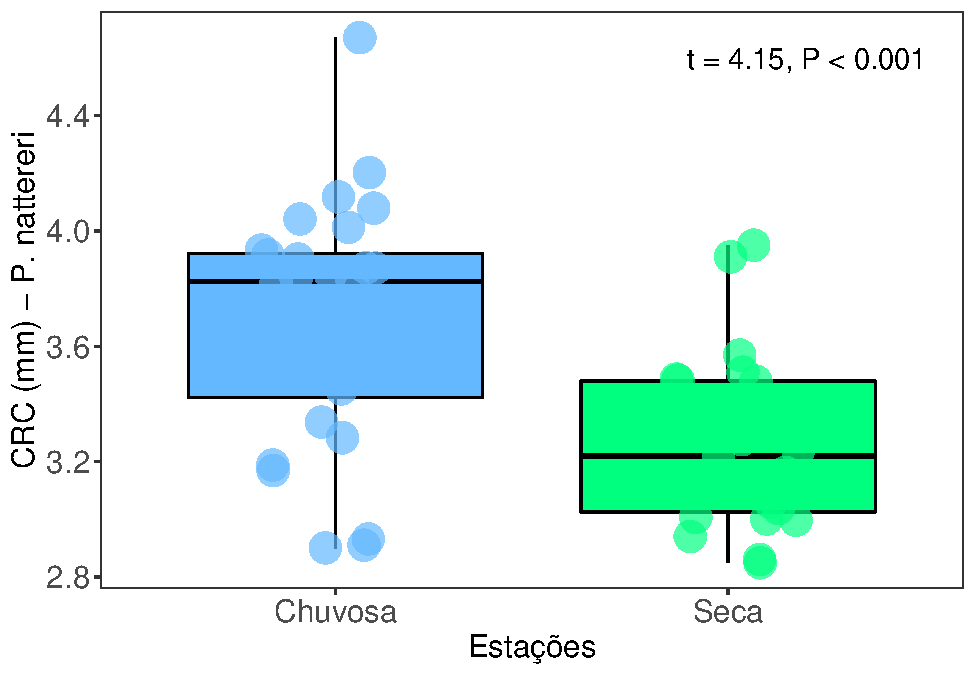
\includegraphics{livro_r_ecologia_files/figure-latex/unnamed-chunk-2-1.pdf}

\hypertarget{interpretauxe7uxe3o-dos-resultados}{%
\subsubsection{Interpretação dos resultados}\label{interpretauxe7uxe3o-dos-resultados}}

Antes de começarmos a interpretar os resultados precisamos verificar que o agrupamento reduziu a dimensionalidade da matiz de forma eficiente, de maneira a não distorcer a informação. Fazemos isso calculando o \textbf{Coeficiente de correlação cofenética (CCC)}

\begin{Shaded}
\begin{Highlighting}[]
\NormalTok{cofresult <-}\StringTok{ }\KeywordTok{cophenetic}\NormalTok{(dendro)}
\KeywordTok{cor}\NormalTok{(cofresult, distBocaina)}
\end{Highlighting}
\end{Shaded}

\begin{verbatim}
## [1] 0.8819701
\end{verbatim}

Um CCC \textgreater{} .7 indica uma boa representação. Portanto, o nosso resultado de 0.8819701 é bastante alto, garantindo que o dendrograma é adequado.

No entanto, para interpretar os resultados precisamos antes definir um nível de corte, que vai nos dizer quantos grupos existem. Há vários métodos para definir grupos, desde os heurísticos aos que utilizam bootstrap. Se quisermos interpretar este dendrograma, podemos por exemplo estabelecer um nível de corte de 50\% de distância (ou seja, grupos cujos objetos tenham ao menos 50\% de similaridade entre si).

\begin{Shaded}
\begin{Highlighting}[]
\KeywordTok{plot}\NormalTok{(dendro)}
\NormalTok{k =}\StringTok{ }\DecValTok{4}
\NormalTok{n =}\StringTok{ }\KeywordTok{nrow}\NormalTok{(bocaina)}
\NormalTok{MidPoint =}\StringTok{ }\NormalTok{(dendro}\OperatorTok{$}\NormalTok{height[n}\OperatorTok{-}\NormalTok{k] }\OperatorTok{+}\StringTok{ }\NormalTok{dendro}\OperatorTok{$}\NormalTok{height[n}\OperatorTok{-}\NormalTok{k}\OperatorTok{+}\DecValTok{1}\NormalTok{]) }\OperatorTok{/}\StringTok{ }\DecValTok{2}
\KeywordTok{abline}\NormalTok{(}\DataTypeTok{h =}\NormalTok{ MidPoint, }\DataTypeTok{lty=}\DecValTok{2}\NormalTok{)}
\end{Highlighting}
\end{Shaded}

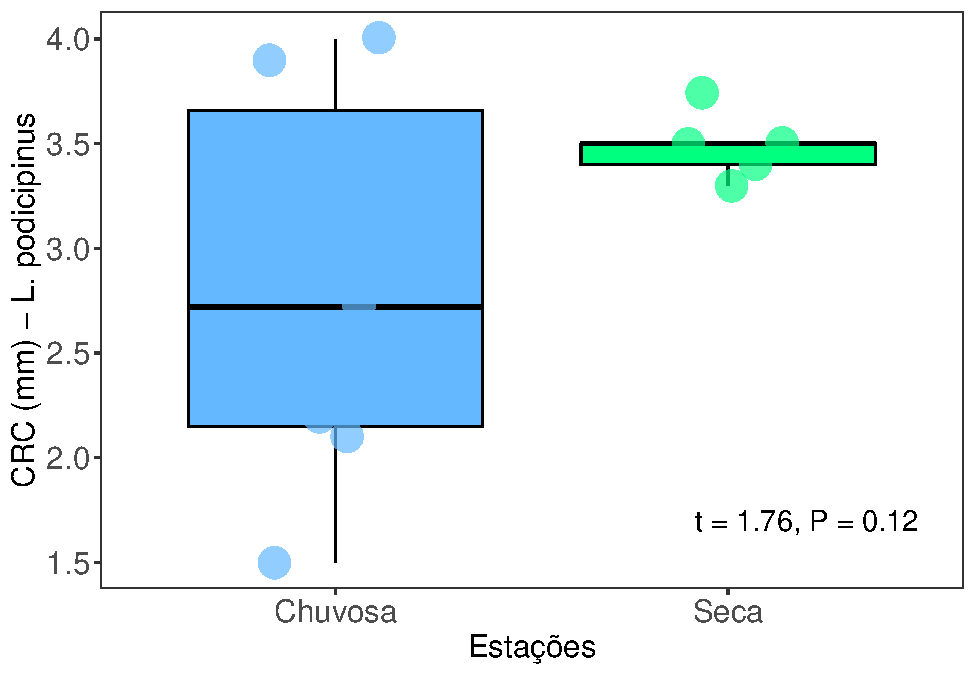
\includegraphics{livro_r_ecologia_files/figure-latex/unnamed-chunk-4-1.pdf}

Nesse caso teremos a formação de cinco grupos, representados pelos nós que estão abaixo da linha de corte.

\hypertarget{exemplo-2}{%
\section{Exemplo 2:}\label{exemplo-2}}

A seguir, vamos utilizar o pacote \texttt{pvclust} que calcula automaticamente o nível de corte de similaridade baseado no Bootstrap de cada nó. Uma desvantagem deste método é que ele somente aceita índices de similaridade da função \texttt{dist} que possui apenas a distância Euclidiana, Manhattan e Canberra. Uma maneira de contornarmos essa limitação é utilizar transformações dos dados disponíveis na função \texttt{disttransform} no pacote \texttt{BiodiversityR} ou o \texttt{decostand} do pacote \texttt{vegan}. Também é possível utilizar a transformação de Box-Cox para dados multivariados, disponível no material suplementar de Legendre \& Borcard (2018) \href{http://www.ecography.org/appendix/ecog-03498}{aqui}

\begin{Shaded}
\begin{Highlighting}[]
\KeywordTok{library}\NormalTok{(pvclust)}
\KeywordTok{library}\NormalTok{(BiodiversityR)}
\end{Highlighting}
\end{Shaded}

Aqui vamos utilizar a distância de Chord para calcular a matriz de distância. Se transformarmos uma matriz usando a transformação Chord e depois calcularmos a distância Euclidiana, isso equivale à calcular diretamente a distância de Chord:

\begin{Shaded}
\begin{Highlighting}[]
\NormalTok{bocaina_transf <-}\StringTok{ }\KeywordTok{disttransform}\NormalTok{(bocaina, }\StringTok{"chord"}\NormalTok{)}
\NormalTok{analise <-}\StringTok{ }\KeywordTok{pvclust}\NormalTok{(bocaina_transf, }\DataTypeTok{method.hclust=}\StringTok{"average"}\NormalTok{, }\DataTypeTok{method.dist=}\StringTok{"euclidean"}\NormalTok{) }
\end{Highlighting}
\end{Shaded}

\begin{verbatim}
## Bootstrap (r = 0.46)... Done.
## Bootstrap (r = 0.54)... Done.
## Bootstrap (r = 0.69)... Done.
## Bootstrap (r = 0.77)... Done.
## Bootstrap (r = 0.85)... Done.
## Bootstrap (r = 1.0)... Done.
## Bootstrap (r = 1.08)... Done.
## Bootstrap (r = 1.15)... Done.
## Bootstrap (r = 1.23)... Done.
## Bootstrap (r = 1.38)... Done.
\end{verbatim}

\begin{Shaded}
\begin{Highlighting}[]
\KeywordTok{plot}\NormalTok{(analise, }\DataTypeTok{hang=}\OperatorTok{-}\DecValTok{1}\NormalTok{)}
\KeywordTok{pvrect}\NormalTok{(analise)}
\end{Highlighting}
\end{Shaded}

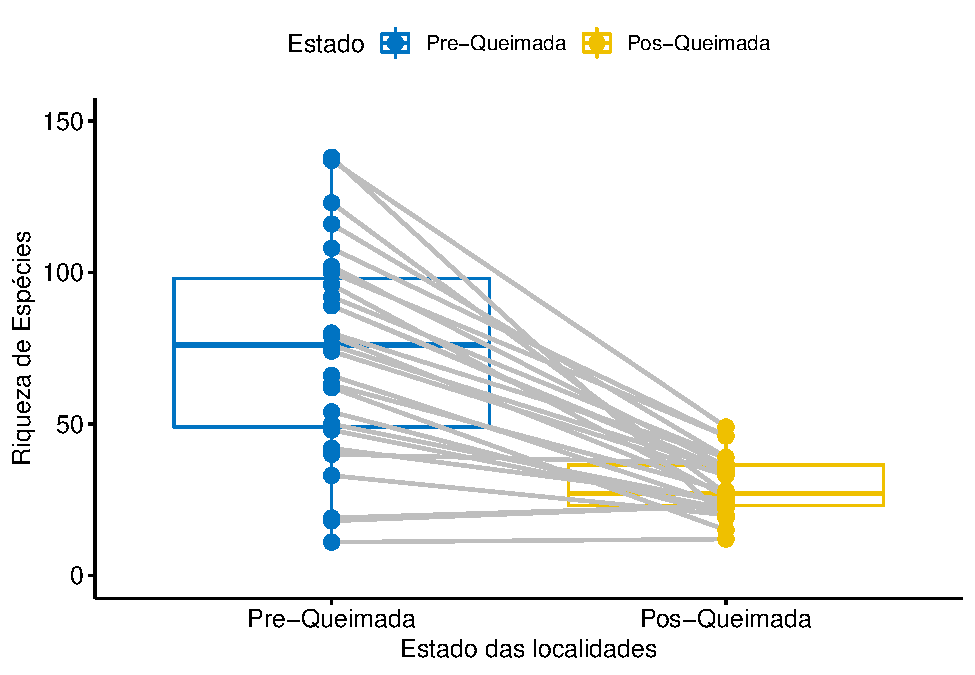
\includegraphics{livro_r_ecologia_files/figure-latex/unnamed-chunk-6-1.pdf}

É possível notar que existe um único grupo com BS \textgreater{} 95\%. Agora vamos tentar usar a distância de Hellinger:

\begin{Shaded}
\begin{Highlighting}[]
\NormalTok{bocaina_transf2 <-}\StringTok{ }\KeywordTok{disttransform}\NormalTok{(bocaina, }\StringTok{"hellinger"}\NormalTok{)}
\NormalTok{analise2 <-}\StringTok{ }\KeywordTok{pvclust}\NormalTok{(bocaina_transf2, }\DataTypeTok{method.hclust=}\StringTok{"average"}\NormalTok{, }\DataTypeTok{method.dist=}\StringTok{"euclidean"}\NormalTok{) }
\end{Highlighting}
\end{Shaded}

\begin{verbatim}
## Bootstrap (r = 0.46)... Done.
## Bootstrap (r = 0.54)... Done.
## Bootstrap (r = 0.69)... Done.
## Bootstrap (r = 0.77)... Done.
## Bootstrap (r = 0.85)... Done.
## Bootstrap (r = 1.0)... Done.
## Bootstrap (r = 1.08)... Done.
## Bootstrap (r = 1.15)... Done.
## Bootstrap (r = 1.23)... Done.
## Bootstrap (r = 1.38)... Done.
\end{verbatim}

\begin{Shaded}
\begin{Highlighting}[]
\KeywordTok{plot}\NormalTok{(analise2, }\DataTypeTok{hang=}\OperatorTok{-}\DecValTok{1}\NormalTok{)}
\KeywordTok{pvrect}\NormalTok{(analise2)}
\end{Highlighting}
\end{Shaded}

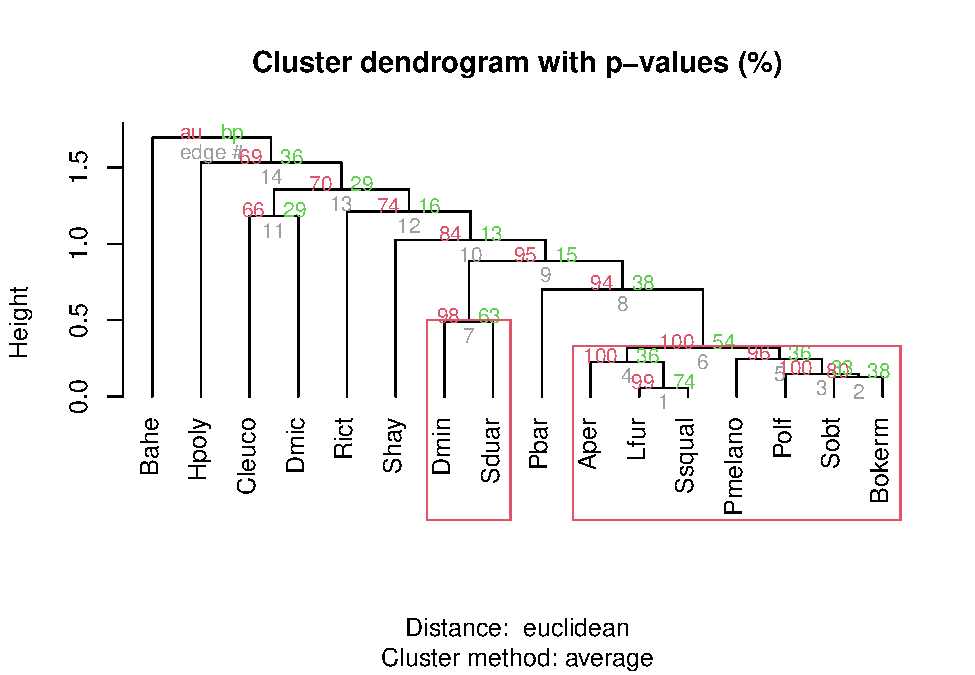
\includegraphics{livro_r_ecologia_files/figure-latex/unnamed-chunk-7-1.pdf}

Notem que se mudarmos o coeficiente de associação, o resultado também muda. Agora temos 1 grupo a mais, composto por \emph{Dendropsophus minutus} e \emph{Scinax duartei} que não apareciam antes. Isso se deve ao fato de que a distância de Hellinger dá menos peso para espécies raras do que a Chord.

\hypertarget{k-means-e-agrupamentos-nuxe3o-hierarquicos}{%
\chapter{K-means e agrupamentos não-hierarquicos}\label{k-means-e-agrupamentos-nuxe3o-hierarquicos}}

\hypertarget{backgorund-da-anuxe1lise-1}{%
\section{Backgorund da análise}\label{backgorund-da-anuxe1lise-1}}

K-means é um tipo de agrupamento não hierarquico porque não busca obter grupos menores que por sua vez pertencem a grupos maiores. Resumidamente, podemos calcular o K-means apartir de uma matriz quadrada ou de distância. Essa técnica procura particionar os objetos em \emph{k} grupos de maneira a minimizar a soma de quadrados entre grupos e maximizá-la dentro dos grupos. Um critério similar ao de uma ANOVA.

\hypertarget{exemplo-1-1}{%
\section{Exemplo 1:}\label{exemplo-1-1}}

\textbf{Pergunta:}

\begin{quote}
Qual é o número de grupos que melhor sumariza o padrão de ocorrência de espécies de peixes ao longo de um riacho?
\end{quote}

\textbf{Predições}

\begin{quote}
\begin{itemize}
\tightlist
\item
  1: O agrupamento ideal para explicar a variância no padrão de ocorrência de espécies é 4.
\end{itemize}
\end{quote}

\textbf{Variáveis}

\begin{itemize}
\tightlist
\item
  Variáveis resposta

  \begin{itemize}
  \item
    \begin{enumerate}
    \def\labelenumi{\arabic{enumi}.}
    \tightlist
    \item
      Para este exemplo iremos utilizar um conjunto de dados disponível no pacote \texttt{ade4} que contém dados de 27 espécies de peixes coletados em 30 pontos ao longo do Rio Doubs, na fronteira entre a França e Suiça.
    \end{enumerate}
  \end{itemize}
\end{itemize}

\hypertarget{explicauxe7uxe3o-da-anuxe1lise-1}{%
\subsection{Explicação da análise}\label{explicauxe7uxe3o-da-anuxe1lise-1}}

Um diferencial do K-means em relação aos agrupamentos hierarquicos (=clusters) é que o usuário pode escolher antecipadamente o número de grupos que quer formar.

\textbf{Checklist}

\begin{itemize}
\tightlist
\item
  Vamos normalizar os dados de abundância antes de entrar na análise propriamente, já que existem muitos zeros na matriz.
\end{itemize}

\hypertarget{anuxe1lise-1}{%
\subsection{Análise}\label{anuxe1lise-1}}

\begin{Shaded}
\begin{Highlighting}[]
\KeywordTok{library}\NormalTok{(ade4)}
\KeywordTok{data}\NormalTok{(doubs)}
\KeywordTok{head}\NormalTok{(doubs}\OperatorTok{$}\NormalTok{fish)}
\end{Highlighting}
\end{Shaded}

\begin{verbatim}
##   Cogo Satr Phph Neba Thth Teso Chna Chto Lele Lece Baba Spbi Gogo Eslu Pefl
## 1    0    3    0    0    0    0    0    0    0    0    0    0    0    0    0
## 2    0    5    4    3    0    0    0    0    0    0    0    0    0    0    0
## 3    0    5    5    5    0    0    0    0    0    0    0    0    0    1    0
## 4    0    4    5    5    0    0    0    0    0    1    0    0    1    2    2
## 5    0    2    3    2    0    0    0    0    5    2    0    0    2    4    4
## 6    0    3    4    5    0    0    0    0    1    2    0    0    1    1    1
##   Rham Legi Scer Cyca Titi Abbr Icme Acce Ruru Blbj Alal Anan
## 1    0    0    0    0    0    0    0    0    0    0    0    0
## 2    0    0    0    0    0    0    0    0    0    0    0    0
## 3    0    0    0    0    0    0    0    0    0    0    0    0
## 4    0    0    0    0    1    0    0    0    0    0    0    0
## 5    0    0    2    0    3    0    0    0    5    0    0    0
## 6    0    0    0    0    2    0    0    0    1    0    0    0
\end{verbatim}

\begin{Shaded}
\begin{Highlighting}[]
\NormalTok{spe <-}\StringTok{ }\NormalTok{doubs}\OperatorTok{$}\NormalTok{fish[}\OperatorTok{-}\DecValTok{8}\NormalTok{,]}\CommentTok{# retiro a linha 8, pois não há dados}
\NormalTok{spe.norm <-}\StringTok{ }\KeywordTok{decostand}\NormalTok{(spe, }\StringTok{"normalize"}\NormalTok{) }\CommentTok{# função do pacote vegan, ela faz várias padronizações, aqui ele normaliza  }
\end{Highlighting}
\end{Shaded}

O argumento \texttt{centers} na função abaixo indica o número de grupos que se quer formar. Neste exemplo estamos utilizando \texttt{centers=4}.

\begin{Shaded}
\begin{Highlighting}[]
\NormalTok{spe.kmeans <-}\StringTok{ }\KeywordTok{kmeans}\NormalTok{(spe.norm, }\DataTypeTok{centers=}\DecValTok{4}\NormalTok{, }\DataTypeTok{nstart=}\DecValTok{100}\NormalTok{)}
\NormalTok{spe.kmeans}
\end{Highlighting}
\end{Shaded}

\begin{verbatim}
## K-means clustering with 4 clusters of sizes 8, 12, 3, 6
## 
## Cluster means:
##         Cogo        Satr       Phph       Neba        Thth        Teso
## 1 0.00000000 0.006691097 0.02506109 0.06987391 0.006691097 0.006691097
## 2 0.10380209 0.542300691 0.50086515 0.43325916 0.114024105 0.075651573
## 3 0.00000000 0.000000000 0.00000000 0.00000000 0.000000000 0.000000000
## 4 0.06167791 0.122088022 0.26993915 0.35942538 0.032664966 0.135403325
##         Chna       Chto       Lele      Lece       Baba      Spbi       Gogo
## 1 0.10687104 0.09377516 0.14194394 0.2011411 0.24327992 0.1326062 0.28386032
## 2 0.00000000 0.00000000 0.06983991 0.1237394 0.02385019 0.0000000 0.05670453
## 3 0.05205792 0.00000000 0.07647191 0.3166705 0.00000000 0.0000000 0.20500174
## 4 0.06212775 0.21568957 0.25887226 0.2722562 0.15647062 0.1574388 0.16822286
##         Eslu       Pefl      Rham       Legi       Scer       Cyca       Titi
## 1 0.20630360 0.16920496 0.2214275 0.19066542 0.13171275 0.16019126 0.26230024
## 2 0.04722294 0.02949244 0.0000000 0.00000000 0.00000000 0.00000000 0.03833408
## 3 0.07647191 0.00000000 0.0000000 0.05205792 0.07647191 0.00000000 0.00000000
## 4 0.12276089 0.17261621 0.0793181 0.06190283 0.04516042 0.06190283 0.14539027
##         Abbr      Icme       Acce       Ruru       Blbj      Alal       Anan
## 1 0.19561641 0.1331835 0.26713081 0.32103755 0.22883055 0.3326939 0.18873077
## 2 0.00000000 0.0000000 0.00000000 0.01049901 0.00000000 0.0000000 0.00000000
## 3 0.00000000 0.0000000 0.18058775 0.31667052 0.05205792 0.7618709 0.00000000
## 4 0.01473139 0.0000000 0.03192175 0.32201597 0.01473139 0.1095241 0.04739636
## 
## Clustering vector:
##  1  2  3  4  5  6  7  9 10 11 12 13 14 15 16 17 18 19 20 21 22 23 24 25 26 27 
##  2  2  2  2  4  2  2  4  2  2  2  2  2  2  4  4  4  4  1  1  1  3  3  3  1  1 
## 28 29 30 
##  1  1  1 
## 
## Within cluster sum of squares by cluster:
## [1] 0.4696535 2.5101386 0.3560423 1.7361453
##  (between_SS / total_SS =  66.7 %)
## 
## Available components:
## 
## [1] "cluster"      "centers"      "totss"        "withinss"     "tot.withinss"
## [6] "betweenss"    "size"         "iter"         "ifault"
\end{verbatim}

O objeto que fornece o resultado contém: 1) o tamanho (número de objetos) em cada um dos 4 grupos; 2) o centroid de cada grupo e o pertencimento de cada espécie a cada grupo; e 3) o quando da Soma de Quadrados dos dados é explicada por esta conformação de grupos.

No entanto, não é possível saber a priori qual o número \emph{ideal} de grupos. Para descobrir isso repetimos o k-means com uma série de valores de \textbf{K}. Isso pode ser feito na função \texttt{cascadeKM}.

\begin{Shaded}
\begin{Highlighting}[]
\NormalTok{spe.KM.cascade <-}\StringTok{ }\KeywordTok{cascadeKM}\NormalTok{(spe.norm, }\DataTypeTok{inf.gr=}\DecValTok{2}\NormalTok{, }\DataTypeTok{sup.gr=}\DecValTok{10}\NormalTok{, }\DataTypeTok{iter=}\DecValTok{100}\NormalTok{, }\DataTypeTok{criterion=}\StringTok{"ssi"}\NormalTok{) }
\end{Highlighting}
\end{Shaded}

Tanto \textbf{calinski} quando \textbf{ssi} são bons critérios para encontrar o número ideal de grupos. Quanto maior o valor de \textbf{ssi} melhor (veja \texttt{?cascadeKM} mais detalhes).

\begin{Shaded}
\begin{Highlighting}[]
\CommentTok{# summary}
\NormalTok{spe.KM.cascade}\OperatorTok{$}\NormalTok{results}
\end{Highlighting}
\end{Shaded}

\begin{verbatim}
##      2 groups  3 groups  4 groups   5 groups   6 groups  7 groups  8 groups
## SSE 8.2149405 6.4768108 5.0719796 4.30155732 3.58561200 2.9523667 2.4840549
## ssi 0.1312111 0.1685126 0.1398159 0.06144551 0.08127954 0.1232942 0.1369294
##       9 groups 10 groups
## SSE 2.05218880 1.7599292
## ssi 0.07877382 0.1081304
\end{verbatim}

SSE: critério utilizado pelo algorítimo para achar o agrupamento ótimo dos objetos.

\begin{Shaded}
\begin{Highlighting}[]
\KeywordTok{plot}\NormalTok{(spe.KM.cascade, }\DataTypeTok{sortg=}\OtherTok{TRUE}\NormalTok{)}
\end{Highlighting}
\end{Shaded}

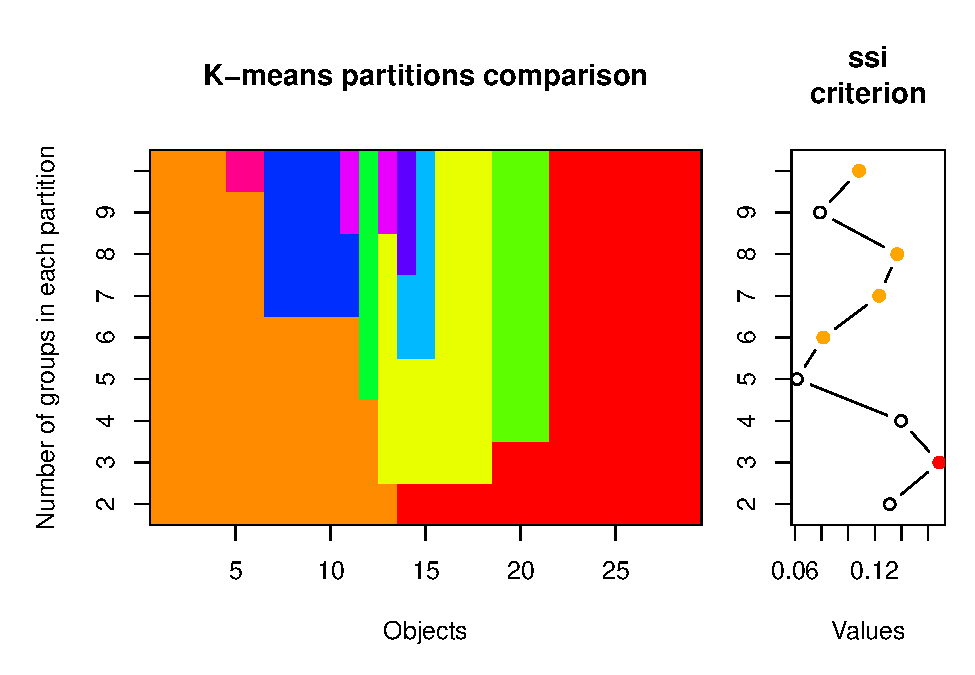
\includegraphics{livro_r_ecologia_files/figure-latex/unnamed-chunk-12-1.pdf}

Este resultado nos mostra que o número ideal de grupos é 3, vejam que o SSI máximo é alcançado neste número de grupos 0.1685126 (também indicado pela bola vermelha no plot).

\#Espécies indicadoras

\hypertarget{backgorund-da-anuxe1lise-2}{%
\section{Backgorund da análise}\label{backgorund-da-anuxe1lise-2}}

Uma pergunta normalmente feita por ecólogos é: qual espécie pode ser indicadora de uma determinada condição ambiental?

O índice IndVal mede dois aspectos das espécies: Especificidade e fidelidade. Uma alta fidelidade significa que espécies ocorrem em todos os locais do grupo e uma alta especificidade significa que as espécies ocorrem somente naquele grupo. Uma boa espécie indicadora é aquela na qual todos os indivíduos ocorrem em todas a amostras referentes a um grupo específico.
A Especificidade é dada pela divisão da abundancia média da espécie no grupo pela somatória das abundancias médias dos grupos. Fidelidade é igual ao número de lugares no grupo onde a espécie está presente dividido pelo número total de lugares do grupo (Dufrêne \& Legendre, 1997).

Espécies raras podem receber o mesmo valor de IndVal das espécies indicadoras e são chamadas de indicadoras assimétricas, i.e., contribuem com a especificidade do habitat mas não servem para predizer grupos. Ao contrário, as espécies indicadoras são verdadeiros indicadores simétricos e podem ser usadas para predizer grupos.

\hypertarget{exemplo-1-2}{%
\section{Exemplo 1:}\label{exemplo-1-2}}

\textbf{Pergunta:}

\begin{quote}
Qual espécie de anfíbio anuro na fase larval pode ser indicadora da fitofisionomia onde é encontrada?
\end{quote}

\textbf{Predições}

\begin{quote}
\begin{itemize}
\tightlist
\item
  1: Espécies terrestres serão indicadoras de área aberta, enquanto espécies arborícolas serão indicadoras de áreas florestais.
\end{itemize}
\end{quote}

\textbf{Variáveis}

\begin{itemize}
\tightlist
\item
  Variáveis resposta

  \begin{itemize}
  \item
    \begin{enumerate}
    \def\labelenumi{\arabic{enumi}.}
    \tightlist
    \item
      Mesma matriz já utilizada contendo a abundância de girinos ao longo de poças na Serra da Bocaina.
    \end{enumerate}
  \end{itemize}
\end{itemize}

\hypertarget{explicauxe7uxe3o-da-anuxe1lise-2}{%
\subsection{Explicação da análise}\label{explicauxe7uxe3o-da-anuxe1lise-2}}

A análise procede da seguinte forma:

\begin{itemize}
\item
  \begin{enumerate}
  \def\labelenumi{\arabic{enumi}.}
  \tightlist
  \item
    Uma matriz de distância é construída e as unidades amostrais são classificadas com alguma análise de agrupamento, hierárquico ou não;
  \end{enumerate}
\item
  \begin{enumerate}
  \def\labelenumi{\arabic{enumi}.}
  \setcounter{enumi}{1}
  \tightlist
  \item
    A variável ambiental para a qual se deseja classificar os grupos é inserida;
  \end{enumerate}
\item
  \begin{enumerate}
  \def\labelenumi{\arabic{enumi}.}
  \setcounter{enumi}{2}
  \tightlist
  \item
    As espécies indicadoreas de cada grupo são formadas através do cálculo da especificidade e fidelidade, obtendo-se o valor de IndVal para cada espécie;
  \end{enumerate}
\item
  \begin{enumerate}
  \def\labelenumi{\arabic{enumi}.}
  \setcounter{enumi}{3}
  \tightlist
  \item
    Por fim, o conjunto de dados originais é comparado para ver se análise faz sentido.
  \end{enumerate}
\end{itemize}

O cálculo da significância do índice de IndVal é feito por aleatorização de Monte Carlo. Assim, o valor do índice é aleatorizado 999 vezes (ou o número de vezes que você optar) dentro dos tratamentos e o valor de \emph{P} é dado pelo número de vezes em que o índice observado foi igual ou maior que os valores aleatorizados.

\hypertarget{anuxe1lise-2}{%
\subsection{Análise}\label{anuxe1lise-2}}

O IndVal está disponível tanto no pacote \texttt{indicspecies} quando no \texttt{labdsv}. Para este exemplo iremos usar o labdsv.

\begin{Shaded}
\begin{Highlighting}[]
\KeywordTok{library}\NormalTok{(labdsv)}
\end{Highlighting}
\end{Shaded}

Primeiro vamos agrupar as unidades amostrais (poças) que informa os grupos de fitofisionomias onde as poças se localizam e para os quais deseja-se encontrar espécies indicadoras:

\begin{Shaded}
\begin{Highlighting}[]
\NormalTok{fitofis <-}\StringTok{ }\KeywordTok{c}\NormalTok{(}\KeywordTok{rep}\NormalTok{(}\DecValTok{1}\NormalTok{,}\DecValTok{4}\NormalTok{), }\KeywordTok{rep}\NormalTok{(}\DecValTok{2}\NormalTok{,}\DecValTok{4}\NormalTok{), }\KeywordTok{rep}\NormalTok{(}\DecValTok{3}\NormalTok{,}\DecValTok{4}\NormalTok{), }\KeywordTok{rep}\NormalTok{(}\DecValTok{4}\NormalTok{,}\DecValTok{4}\NormalTok{), }\KeywordTok{rep}\NormalTok{(}\DecValTok{5}\NormalTok{,}\DecValTok{4}\NormalTok{))}
\end{Highlighting}
\end{Shaded}

\begin{Shaded}
\begin{Highlighting}[]
\NormalTok{resultado <-}\StringTok{ }\KeywordTok{indval}\NormalTok{(bocaina, fitofis)}
\KeywordTok{summary}\NormalTok{(resultado)}\CommentTok{#só exibe o resultado para as espécies indicadoras}
\end{Highlighting}
\end{Shaded}

\begin{verbatim}
##       cluster indicator_value probability
## Rict        1          0.8364       0.010
## Sduar       1          0.7475       0.047
## 
## Sum of probabilities                 =  8.047 
## 
## Sum of Indicator Values              =  7.3 
## 
## Sum of Significant Indicator Values  =  1.58 
## 
## Number of Significant Indicators     =  2 
## 
## Significant Indicator Distribution
## 
## 1 
## 2
\end{verbatim}

Para apresentar uma tabela dos resultados para todas as espécies temos de processar os dados:

\begin{Shaded}
\begin{Highlighting}[]
\NormalTok{resultado}\OperatorTok{$}\NormalTok{maxcls}
\end{Highlighting}
\end{Shaded}

\begin{verbatim}
##    Aper    Bahe    Rict  Cleuco    Dmic    Dmin   Hpoly    Lfur    Pbar    Polf 
##       3       2       1       3       3       1       2       3       1       3 
## Pmelano   Sduar    Shay    Sobt  Ssqual  Bokerm 
##       2       1       3       2       3       2
\end{verbatim}

\begin{Shaded}
\begin{Highlighting}[]
\NormalTok{resultado}\OperatorTok{$}\NormalTok{indcls}
\end{Highlighting}
\end{Shaded}

\begin{verbatim}
##      Aper      Bahe      Rict    Cleuco      Dmic      Dmin     Hpoly      Lfur 
## 0.2432796 0.6487329 0.8363823 0.4128631 0.6645244 0.7032145 0.6208711 0.2279412 
##      Pbar      Polf   Pmelano     Sduar      Shay      Sobt    Ssqual    Bokerm 
## 0.2813725 0.2437500 0.2500000 0.7474527 0.4930269 0.2222222 0.2500000 0.4583333
\end{verbatim}

\begin{Shaded}
\begin{Highlighting}[]
\NormalTok{resultado}\OperatorTok{$}\NormalTok{pval}
\end{Highlighting}
\end{Shaded}

\begin{verbatim}
##    Aper    Bahe    Rict  Cleuco    Dmic    Dmin   Hpoly    Lfur    Pbar    Polf 
##   1.000   0.060   0.010   0.395   0.238   0.084   0.266   1.000   0.585   1.000 
## Pmelano   Sduar    Shay    Sobt  Ssqual  Bokerm 
##   1.000   0.047   0.423   0.710   1.000   0.229
\end{verbatim}

\begin{Shaded}
\begin{Highlighting}[]
\NormalTok{tab.resultado=}\KeywordTok{cbind}\NormalTok{(resultado}\OperatorTok{$}\NormalTok{maxcls,resultado}\OperatorTok{$}\NormalTok{indcls,resultado}\OperatorTok{$}\NormalTok{pval)}
\KeywordTok{colnames}\NormalTok{(tab.resultado)<-}\KeywordTok{c}\NormalTok{(}\StringTok{"maxgrp"}\NormalTok{, }\StringTok{"ind. value"}\NormalTok{,}\StringTok{"P"}\NormalTok{)}
\NormalTok{tab.resultado}
\end{Highlighting}
\end{Shaded}

\begin{verbatim}
##         maxgrp ind. value     P
## Aper         3  0.2432796 1.000
## Bahe         2  0.6487329 0.060
## Rict         1  0.8363823 0.010
## Cleuco       3  0.4128631 0.395
## Dmic         3  0.6645244 0.238
## Dmin         1  0.7032145 0.084
## Hpoly        2  0.6208711 0.266
## Lfur         3  0.2279412 1.000
## Pbar         1  0.2813725 0.585
## Polf         3  0.2437500 1.000
## Pmelano      2  0.2500000 1.000
## Sduar        1  0.7474527 0.047
## Shay         3  0.4930269 0.423
## Sobt         2  0.2222222 0.710
## Ssqual       3  0.2500000 1.000
## Bokerm       2  0.4583333 0.229
\end{verbatim}

No resultado podemos ver que temos duas espécies indicadoras da fitofisionimia 1: \emph{Rhinella icterica} (Rict) e \emph{Scinax duartei} (Sduar). Nenhuma espécie foi indicadora dos outros grupos neste exemplo.

\hypertarget{para-se-aprofundar}{%
\subsection{Para se aprofundar}\label{para-se-aprofundar}}

\begin{itemize}
\tightlist
\item
  \href{https://www.sciencedirect.com/science/article/pii/S0304380010006393?casa_token=0YLFbVbGj1IAAAAA:RFcrLHBDdt-NY5gpxCEAqlc8LMG0ayzChpMvaOFQkE10ftg2Us6PafgMQCSmCZZ21eb430e_lWo}{Agrupamento de espécies e locais baseado em modelos}
\item
  \href{http://adn.biol.umontreal.ca/~numericalecology/numecolR/}{Numerical Ecology with R}
\end{itemize}

\hypertarget{rarefauxe7uxe3o}{%
\chapter{Rarefação}\label{rarefauxe7uxe3o}}

\hypertarget{background-da-anuxe1lise}{%
\section{Background da análise}\label{background-da-anuxe1lise}}

Uma das dificuldades na comparação da riqueza de espécies entre comunidades é decorrente da diferença no esforço amostral (e.g.diferença no número de indivíduos, discrepância na quantidade de unidades amostrais ou área amostrada) que inevitavelmente influenciará no número de espécies observadas (Gotelli \& Chao 2013). O método de rarefação nos permite comparar o número de espécies entre comunidades quando o tamanho da amostra ou a abundância de indivíduos não são iguais. A rarefação calcula o número esperado de espécies em cada comunidade tendo como base comparativa um valor em que todas as amostras atinjam um tamanho padrão, ou comparações baseadas na comunidade com menor número de amostragens ou com menos indivíduos. O teste foi formulado considerando seguinte pergunta: Se considerarmos \emph{n} indivíduos ou amostras (\emph{n} \textless{} N) para cada comunidade, quantas espécies registraríamos nas comunidades considerando o mesmo número de indivíduos ou amostras?

\[E(S) = \sum 1 - \frac{{(N - N_1)}/{n}}{{N}/{n}}\]

Onde:

\begin{itemize}
\item
  E(S) = Número de espécies esperado,
\item
  N = Número total de indivíduos na amostra,
\item
  Ni = Número de indivíduos da iésima espécie,
\item
  \emph{n} = tamanho da amostra padronizada (menor amostra).
\end{itemize}

Gotelli \& Collwel (2001) descrevem este método e discutem em detalhes as restrições sobre seu uso na ecologia:

\begin{itemize}
\tightlist
\item
  As amostras a serem comparados devem ser consistentes do ponto de vista taxonômico, ou seja, todos os indivíduos devem pertencer ao mesmo grupo taxonômico;\\
\item
  As comparações devem ser realizadas somente entre amostras com as mesmas técnicas de coleta;\\
\item
  Os tipos de hábitat onde as amostras são obtidas devem ser semelhantes;\\
\item
  É um método para estimar a riqueza de espécies em uma amostra menor -- não pode ser usado para extrapolar e estimar riqueza.
\end{itemize}

Contudo, é importante ressaltar que esta última restrição foi superada por Colwell et al.~(2012) e Chao \& Jost (2012) que desenvolveram uma nova abordagem onde os dados podem ser interpolados (rarefeito) para amostras menores e extrapolados para amostras maiores.

\hypertarget{exemplo-pruxe1tico-1---morcegos}{%
\section{Exemplo prático 1 - Morcegos}\label{exemplo-pruxe1tico-1---morcegos}}

\hypertarget{explicauxe7uxe3o}{%
\subsection{Explicação}\label{explicauxe7uxe3o}}

\textbf{Explicação dos dados}

Neste exemplo usaremos os dados de espécies de morcegos amostradas em três fragmentos florestais (Breviglieri 2008): i) Mata Ciliar do Córrego Talhadinho com 12 hectares inserida em uma matriz de pastagem; ii) Mata Ciliar do Córrego dos Tenentes com 10 hectares inserida em uma matriz de cultivo de cana-de-açucar e pastagem; e iii) Fazenda Experimental de Pindorama com 128 hectares inserida uma matriz de cana-de-açúcar e pastagem.

\textbf{Pergunta:}

\begin{quote}
A riqueza de espécies de morcegos é maior na Fazenda Experimental do que nos fragmentos florestais menores?
\end{quote}

\textbf{Predições}

\begin{quote}
O número de espécies será maior em fragmentos florestais maiores.
\end{quote}

\textbf{Variáveis}

\begin{itemize}
\tightlist
\item
  Variáveis preditoras

  \begin{itemize}
  \tightlist
  \item
    matriz ou dataframe com as abundâncias das espécies de morcegos registradas nos três fragmentos florestais
  \end{itemize}
\end{itemize}

\textbf{Checklist}

\begin{itemize}
\tightlist
\item
  Verificar se a sua matriz ou dataframe estão com as espécies nas linhas e os fragmentos florestais nas colunas
\end{itemize}

\hypertarget{anuxe1lise}{%
\subsection{Análise}\label{anuxe1lise}}

Calculo da rarefação

\begin{Shaded}
\begin{Highlighting}[]
\KeywordTok{library}\NormalTok{(iNEXT)}
\KeywordTok{library}\NormalTok{(devtools)}
\NormalTok{devtools}\OperatorTok{::}\KeywordTok{install_github}\NormalTok{(}\StringTok{"paternogbc/ecodados"}\NormalTok{)}
\KeywordTok{library}\NormalTok{(ecodados)}

\NormalTok{dados_rarefacao <-}\StringTok{ }\NormalTok{rarefacao_morcegos}
\NormalTok{resultados_morcegos <-}\StringTok{ }\KeywordTok{iNEXT}\NormalTok{(dados_rarefacao, }\DataTypeTok{q =} \DecValTok{0}\NormalTok{, }\DataTypeTok{datatype =} \StringTok{"abundance"}\NormalTok{, }\DataTypeTok{endpoint =} \DecValTok{800}\NormalTok{)}
\CommentTok{# q refere-se a família *Hill-numbers* (Hill 1973) onde 0 = riqueza de espécies, 1 =  diversidade de Shannon, e 2 = diversidade de Simpson.}
\CommentTok{# Veja mais detalhes sobre os números de Hill no Capítulo 7 onde tratamos de extrapolações.}
\CommentTok{# datatype refere-se ao tipo de dados que você vai analisar (e.g. abudância, incidência).}
\CommentTok{# endpoint refere-se ao valor de referência que você determina para a extrapolação.}

\CommentTok{# Visualizar os resultados }
\KeywordTok{ggiNEXT}\NormalTok{(resultados_morcegos, }\DataTypeTok{type =} \DecValTok{1}\NormalTok{)}
\end{Highlighting}
\end{Shaded}

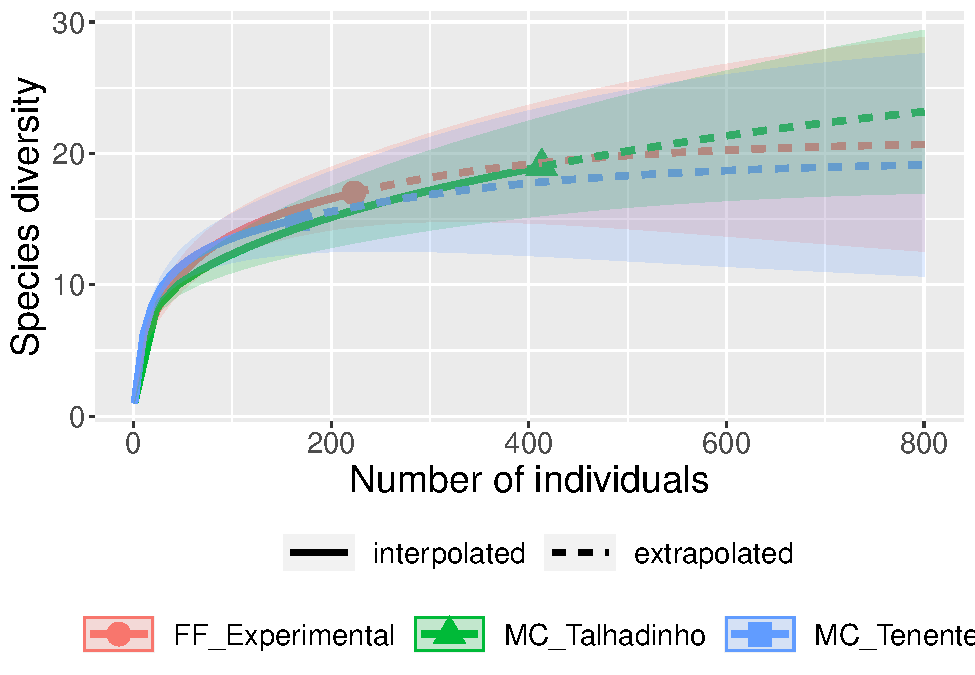
\includegraphics{livro_r_ecologia_files/figure-latex/unnamed-chunk-17-1.pdf}

\hypertarget{interpretauxe7uxe3o-dos-resultados}{%
\subsection{Interpretação dos resultados}\label{interpretauxe7uxe3o-dos-resultados}}

Neste exemplo, foram registrados 166 indivíduos na MC\_Tenentes, 413 na MC\_Talhadinho e 223 na FF\_Experimental. Lembrando, você não pode comparar a riqueza de espécies observada diretamente: 15 espécies na MC\_Tenentes, 17 espécies na MC\_Talhadinho, e 13 espécies no FF\_Experimental. A comparação da riqueza de espécies entre as comunidades deve ser feita com base na riqueza de espécies estimada que é calculada com base no número de indivíduos da comunidade com menor abundância (166 indivíduos). Olhando o gráfico é possível perceber que a riqueza de espécies de morcegos estimada não é diferente entre os três fragmentos florestais quando corrigimos o problema da abundância pela rarefação. A interpretação é feita com base no intervalo de confiança de 95\%. As curvas serão diferentes quando os intervalos de confiança não se sobreporem (Chao et al.~2014). Percebam que está abordagem, além da interpolação (rarefação), também realiza extrapolações que podem ser usadas para estimar o número de espécies caso o esforço de coleta fosse maior. Este é o assunto do nosso próximo capítulo.

~

\hypertarget{exemplo-pruxe1tico-2---rarefauxe7uxe3o}{%
\section{Exemplo prático 2 - Rarefação}\label{exemplo-pruxe1tico-2---rarefauxe7uxe3o}}

\hypertarget{explicauxe7uxe3o-1}{%
\subsection{Explicação}\label{explicauxe7uxe3o-1}}

\textbf{Explicação dos dados}

Neste exemplo iremos comparar o número de espécies de anuros e répteis (serptentes e lagartos) usando informações dos indivíduos depositados em coleções científicas e coletas de campo (da Silva et al.~2017).

\textbf{Pergunta:}

\begin{quote}
A riqueza de espécies de anuros e répteis é maior em coleções científicas do que nas coletas de campo?
\end{quote}

\textbf{Predições}

\begin{quote}
O número de espécies será maior em coleções científicas devido ao maior esforço amostral (i.e.~maior variação temporal para depositar os indíviduos e maior número de pessoas contribuindo com as informações de diferentes estudos e/ou coletas esporádicas).
\end{quote}

\textbf{Variáveis}

\begin{itemize}
\tightlist
\item
  Variáveis preditoras

  \begin{itemize}
  \tightlist
  \item
    matriz ou dataframe com as abundâncias das espécies de anuros e répteis (planilhas separadas) registradas em coleções científicas e coletas de campo.
  \end{itemize}
\end{itemize}

\textbf{Checklist}

\begin{itemize}
\tightlist
\item
  Verificar se a sua matriz ou dataframe estão com as espécies nas linhas e a fonte dos dados nas colunas.
\end{itemize}

\hypertarget{anuxe1lise-1}{%
\subsection{Análise}\label{anuxe1lise-1}}

Calculo da rarefação para os dados de répteis

\begin{Shaded}
\begin{Highlighting}[]
\KeywordTok{library}\NormalTok{(iNEXT)}

\NormalTok{rarefacao_repteis <-}\StringTok{ }\NormalTok{rarefacao_repteis}
\NormalTok{resultados_repteis <-}\StringTok{ }\KeywordTok{iNEXT}\NormalTok{(rarefacao_repteis, }\DataTypeTok{q =} \DecValTok{0}\NormalTok{, }\DataTypeTok{datatype =} \StringTok{"abundance"}\NormalTok{, }\DataTypeTok{endpoint =} \DecValTok{200}\NormalTok{)}

\CommentTok{# Visualizar os resultados }
\KeywordTok{ggiNEXT}\NormalTok{(resultados_repteis, }\DataTypeTok{type =} \DecValTok{1}\NormalTok{)}
\end{Highlighting}
\end{Shaded}

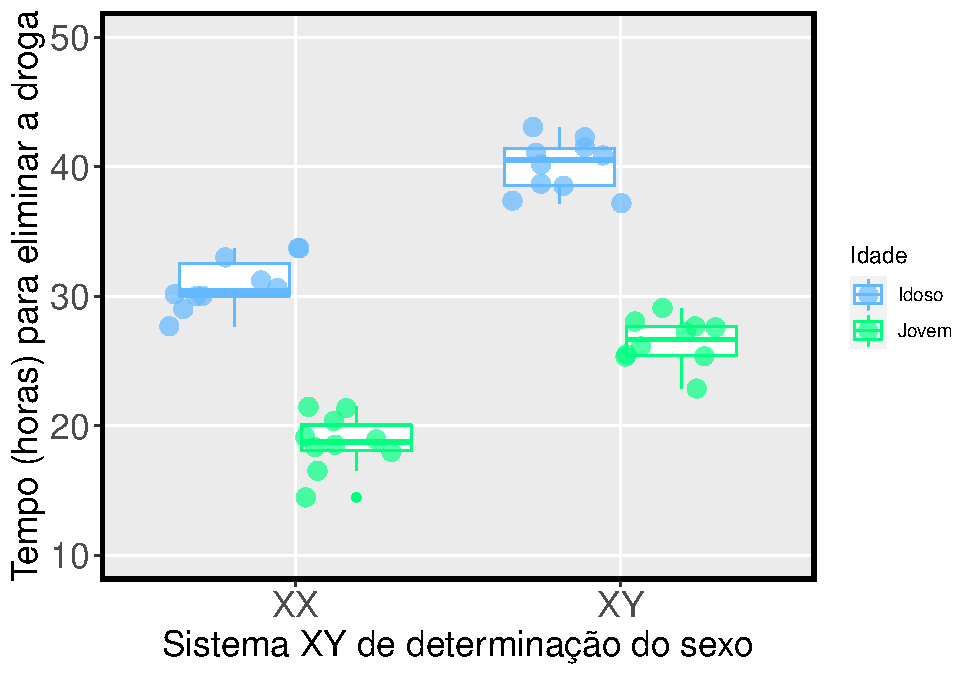
\includegraphics{livro_r_ecologia_files/figure-latex/unnamed-chunk-18-1.pdf}

\hypertarget{interpretauxe7uxe3o-dos-resultados-1}{%
\subsection{Interpretação dos resultados}\label{interpretauxe7uxe3o-dos-resultados-1}}

Neste exemplo,foram registradas oito espécies de répteis nas coletas de campo (40 indivíduos) e 28 espécies nas coleções científicas (77 indivíduos). Com base na rarefação, concluímos que a riqueza de espécies de répteis obtida nas coleções científicas é 2,5 vezes maior do que a obtida em coletas de campo.

~

Calculo da rarefação para os dados dos anuros

\begin{Shaded}
\begin{Highlighting}[]
\KeywordTok{library}\NormalTok{(iNEXT)}

\NormalTok{rarefacao_anuros <-}\StringTok{ }\NormalTok{rarefacao_anuros}
\NormalTok{resultados_anuros <-}\StringTok{ }\KeywordTok{iNEXT}\NormalTok{(rarefacao_anuros, }\DataTypeTok{q =} \DecValTok{0}\NormalTok{, }\DataTypeTok{datatype =} \StringTok{"abundance"}\NormalTok{, }\DataTypeTok{endpoint =} \DecValTok{800}\NormalTok{)}

\CommentTok{# Visualizar os resultados }
\KeywordTok{ggiNEXT}\NormalTok{(resultados_anuros, }\DataTypeTok{type =} \DecValTok{1}\NormalTok{, }\DataTypeTok{grey =} \OtherTok{TRUE}\NormalTok{)}
\end{Highlighting}
\end{Shaded}

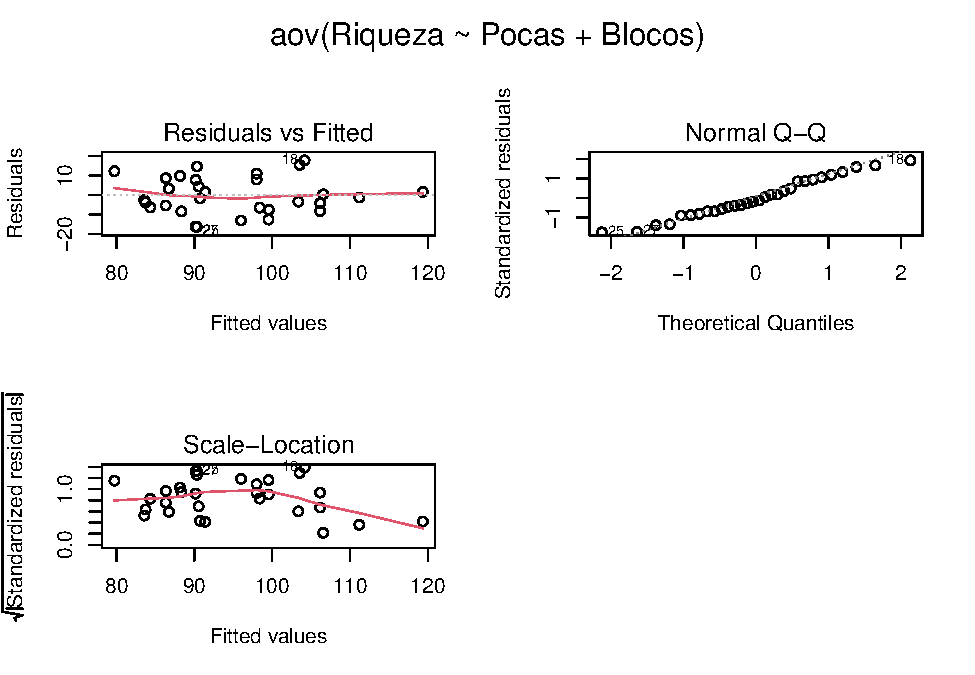
\includegraphics{livro_r_ecologia_files/figure-latex/unnamed-chunk-19-1.pdf}

\textbf{Interpretação dos resultados}

Neste exemplo,foram registradas 21 espécies de anuros nas coletas de campo (709 indivíduos) e 12 espécies nas coleções científicas (37 indivíduos). Com base na rarefação, concluímos que não há diferença entre a riqueza de espécies de anuros obtida em coletas de campo e coleções científicas.

~

\hypertarget{para-se-aprofundar}{%
\section{Para se aprofundar}\label{para-se-aprofundar}}

\begin{itemize}
\item
  Recomendamos aos interessados que olhem a página do \href{http://viceroy.eeb.uconn.edu/estimates}{EstimateS software} e baixem o manual do usuário que contém informações detalhadas sobre os índices de rarefação.Este site foi criado e é mantido pelo Dr.~Robert K. Colwell, um dos maiores especialistas do mundo em estimativas da biodiversidade
\item
  Recomendamos também o livro Magurran \& McGill (2010) - Biological Diversity Frontiers in Measurement and Assessment.
\end{itemize}

\hypertarget{estimadores-de-riqueza}{%
\chapter{Estimadores de Riqueza}\label{estimadores-de-riqueza}}

\hypertarget{backgorund-da-anuxe1lise}{%
\section{Backgorund da análise}\label{backgorund-da-anuxe1lise}}

Uma vez que determinar o número total de espécies numa área é praticamente impossível, principalmente em regiões com alta riqueza de espécies, os estimadores são úteis para extrapolar a riqueza observada e tentar estimar a riqueza total através de uma amostra incompleta de uma comunidade biológica (Walther \& Moore 2005). Neste capítulo serão considerados os estimadores não paramétricos que usam informações da frequencia de espécies raras na comunidade (Gotelli \& Chao 2013). Isto porque tanto os testes paramétricos que tentam determinar os parâmetros de uma curva usando o formato da curva de acumulação de espécies (e.g.~equação logística, Michaelis-Menten) quanto os testes que usam a frequencia do número de indivíduos para enquadrá-las em uma das distribuições de abundância das espécies (e.g.~distribuições log-séries, log-normal) não funcionam muito bem com dados empíricos (Gotelli \& Chao 2013). Para mais detalhes sobre os testes paramétricos veja Magurran (2004) e Colwell (2019).

\begin{quote}
\hypertarget{quatro-caracteruxedsticas-para-um-bom-estimador-de-riqueza-chazdon-et-al.-1998-horter-et-al.-2006}{%
\subsubsection{Quatro características para um bom estimador de riqueza (Chazdon et al.~1998; Horter et al.~2006):}\label{quatro-caracteruxedsticas-para-um-bom-estimador-de-riqueza-chazdon-et-al.-1998-horter-et-al.-2006}}

\begin{itemize}
\tightlist
\item
  Independência do tamanho da amostra (quantidade de esforço amostral realizado);
\item
  Insensibilidade a diferentes padrões de distribuições (diferentes equitabilidades);
\item
  Insensibilidade em relação à ordem das amostragens;
\item
  Insensibilidade à heterogeneidade entre as amostras usadas entre estudos.
\end{itemize}
\end{quote}

\hypertarget{estimadores-baseados-na-abunduxe2ncia-das-espuxe9cies}{%
\section{Estimadores baseados na abundância das espécies}\label{estimadores-baseados-na-abunduxe2ncia-das-espuxe9cies}}

\hypertarget{chao-1---chao-1984-1987}{%
\subsection{CHAO 1 - (Chao 1984, 1987):}\label{chao-1---chao-1984-1987}}

Estimador simples do número absoluto de espécies em uma comunidade. É baseado no número de espécies raras dentro de uma amostra.

\begin{quote}
\[Chao_{1} = S_{obs} + \left(\frac{n-1}{n}\right)\frac{F_1(F_1-1)}{2(F_2+1)}\]
\end{quote}

onde:

\begin{itemize}
\item
  Sobs = o número de espécies na comunidade,
\item
  \emph{n} = número de amostras,
\item
  F1 = número de espécies observadas com abundância de um indivíduo (espécies \emph{singleton}),
\item
  F2 = número de espécies observadas com abundância de dois indivíduos (espécies \emph{doubletons}).
\end{itemize}

O valor de Chao 1 é máximo quando todas as espécies menos uma são únicas (\emph{singleton}). Neste caso, a riqueza estimada é aproximadamente o dobro da riqueza observada.

~

\hypertarget{exemplo-pruxe1tico---chao-1}{%
\subsubsection{Exemplo prático - Chao 1}\label{exemplo-pruxe1tico---chao-1}}

\hypertarget{explicauxe7uxe3o-dos-dados}{%
\paragraph{Explicação dos dados}\label{explicauxe7uxe3o-dos-dados}}

Neste exemplo usaremos os dados de 17 espécies de anuros amostradas em 14 dias de coletas de campo em um habitat reprodutivo localizado na região noroeste do estado de São Paulo, Brasil.

\textbf{Pergunta:}

\begin{quote}
Quantas espécies a mais poderiam ser amostradas caso aumentassemos o esforço amostral?
\end{quote}

\textbf{Predições}

\begin{quote}
\begin{itemize}
\tightlist
\item
  O número de espécies estimadas é similar ao número de espécies observada;
\item
  O número de espécies estimadas é maior do que o número de espécies observada.
\end{itemize}
\end{quote}

\textbf{Variáveis}

\begin{itemize}
\tightlist
\item
  Variáveis preditoras

  \begin{itemize}
  \tightlist
  \item
    matriz ou vetor com as abundâncias das espécies de anuros registradas em um habitat reprodutivo
  \end{itemize}
\end{itemize}

\textbf{Checklist}

\begin{itemize}
\tightlist
\item
  Verificar se a sua matriz está com as espécies nas colunas e as amostragens nas linhas
\item
  Verificar se os dados são de abundância e não presença e ausência
\end{itemize}

\hypertarget{anuxe1lise}{%
\subsection{Análise}\label{anuxe1lise}}

Calculo do estimador de riqueza - Chao 1

\begin{Shaded}
\begin{Highlighting}[]
\KeywordTok{library}\NormalTok{(ecodados)}
\KeywordTok{library}\NormalTok{(vegan)}
\NormalTok{dados_coleta <-}\StringTok{ }\NormalTok{poca_anuros}
\NormalTok{est_chao1 <-}\StringTok{ }\KeywordTok{estaccumR}\NormalTok{(dados_coleta, }\DataTypeTok{permutations =} \DecValTok{100}\NormalTok{)}
\KeywordTok{summary}\NormalTok{(est_chao1, }\DataTypeTok{display =} \StringTok{"chao"}\NormalTok{)}
\end{Highlighting}
\end{Shaded}

\begin{verbatim}
## $chao
##         N      Chao 2.5%    97.5%  Std.Dev
## Dia_3   1  7.086667  4.0 12.33333 2.518671
## Dia_9   2  9.497667  6.0 15.52500 2.358165
## Dia_13  3 11.050000  8.0 16.75000 2.600586
## Dia_5   4 12.012500  9.0 16.00000 2.191210
## Dia_4   5 12.989167  9.0 18.00000 2.446614
## Dia_8   6 13.912500 10.0 22.00000 2.634523
## Dia_14  7 14.830000 11.0 22.00000 2.765425
## Dia_12  8 15.595000 11.0 22.00000 2.887651
## Dia_6   9 16.278333 12.0 22.00000 2.809222
## Dia_11 10 17.095000 13.0 22.00000 2.705863
## Dia_7  11 17.905000 13.0 22.00000 2.654037
## Dia_10 12 18.840000 15.0 22.00000 2.207517
## Dia_2  13 19.535000 15.5 22.00000 1.586329
## Dia_1  14 20.000000 20.0 20.00000 0.000000
## 
## attr(,"class")
## [1] "summary.poolaccum"
\end{verbatim}

Visualizar os resultados com intervalo de confiança de 95\%.

\begin{Shaded}
\begin{Highlighting}[]
\KeywordTok{library}\NormalTok{(ggplot2)}
\CommentTok{# preparando os dados para fazer o gráfico}
\NormalTok{resultados <-}\StringTok{ }\KeywordTok{summary}\NormalTok{(est_chao1, }\DataTypeTok{display =} \KeywordTok{c}\NormalTok{(}\StringTok{"S"}\NormalTok{, }\StringTok{"chao"}\NormalTok{))}
\NormalTok{res_chao <-}\StringTok{ }\KeywordTok{cbind}\NormalTok{(resultados}\OperatorTok{$}\NormalTok{chao[,}\DecValTok{1}\OperatorTok{:}\DecValTok{4}\NormalTok{], resultados}\OperatorTok{$}\NormalTok{S[,}\DecValTok{2}\OperatorTok{:}\DecValTok{4}\NormalTok{])}
\NormalTok{res_chao <-}\StringTok{ }\KeywordTok{as.data.frame}\NormalTok{(res_chao)}
\KeywordTok{colnames}\NormalTok{(res_chao) <-}\StringTok{ }\KeywordTok{c}\NormalTok{(}\StringTok{"Amostras"}\NormalTok{, }\StringTok{"Chao"}\NormalTok{, }\StringTok{"C_inferior"}\NormalTok{, }\StringTok{"C_superior"}\NormalTok{, }\StringTok{"Riqueza"}\NormalTok{,}
                        \StringTok{"R_inferior"}\NormalTok{, }\StringTok{"R_superior"}\NormalTok{)}

\CommentTok{# comando para o gráfico}
\KeywordTok{ggplot}\NormalTok{(res_chao, }\KeywordTok{aes}\NormalTok{(}\DataTypeTok{y =}\NormalTok{ Riqueza, }\DataTypeTok{x =}\NormalTok{ Amostras)) }\OperatorTok{+}
\StringTok{  }\KeywordTok{geom_point}\NormalTok{(}\KeywordTok{aes}\NormalTok{(}\DataTypeTok{y =}\NormalTok{ Chao, }\DataTypeTok{x =}\NormalTok{ Amostras }\OperatorTok{+}\StringTok{ }\FloatTok{0.1}\NormalTok{), }\DataTypeTok{size =} \DecValTok{5}\NormalTok{, }\DataTypeTok{color =} \StringTok{"blue"}\NormalTok{, }\DataTypeTok{alpha =} \DecValTok{1}\NormalTok{) }\OperatorTok{+}
\StringTok{  }\KeywordTok{geom_point}\NormalTok{(}\KeywordTok{aes}\NormalTok{(}\DataTypeTok{y =}\NormalTok{ Riqueza, }\DataTypeTok{x =}\NormalTok{ Amostras), }\DataTypeTok{size =} \DecValTok{5}\NormalTok{, }\DataTypeTok{color =} \StringTok{"red"}\NormalTok{, }\DataTypeTok{alpha =} \DecValTok{1}\NormalTok{) }\OperatorTok{+}
\StringTok{  }\KeywordTok{geom_line}\NormalTok{ (}\KeywordTok{aes}\NormalTok{(}\DataTypeTok{y =}\NormalTok{ Chao, }\DataTypeTok{x =}\NormalTok{ Amostras), }\DataTypeTok{color =} \StringTok{"blue"}\NormalTok{) }\OperatorTok{+}
\StringTok{  }\KeywordTok{geom_line}\NormalTok{ (}\KeywordTok{aes}\NormalTok{(}\DataTypeTok{y =}\NormalTok{ Riqueza, }\DataTypeTok{x =}\NormalTok{ Amostras), }\DataTypeTok{color =} \StringTok{"red"}\NormalTok{) }\OperatorTok{+}
\StringTok{  }\KeywordTok{geom_linerange}\NormalTok{(}\KeywordTok{aes}\NormalTok{(}\DataTypeTok{ymin =}\NormalTok{ C_inferior, }\DataTypeTok{ymax =}\NormalTok{ C_superior, }\DataTypeTok{x =}\NormalTok{ Amostras }\OperatorTok{+}\StringTok{ }\FloatTok{0.1}\NormalTok{),}
 \DataTypeTok{color =} \StringTok{"blue"}\NormalTok{) }\OperatorTok{+}
\StringTok{  }\KeywordTok{geom_linerange}\NormalTok{(}\KeywordTok{aes}\NormalTok{(}\DataTypeTok{ymin =}\NormalTok{ R_inferior, }\DataTypeTok{ymax =}\NormalTok{ R_superior, }\DataTypeTok{x =}\NormalTok{ Amostras), }\DataTypeTok{color =} \StringTok{"red"}\NormalTok{) }\OperatorTok{+}
\StringTok{  }\KeywordTok{ylab}\NormalTok{ (}\StringTok{"Estimador de riqueza - Chao 1"}\NormalTok{) }\OperatorTok{+}
\StringTok{  }\KeywordTok{xlab}\NormalTok{ (}\StringTok{"Número de amostras"}\NormalTok{) }\OperatorTok{+}
\StringTok{  }\KeywordTok{scale_x_continuous}\NormalTok{(}\DataTypeTok{limits =} \KeywordTok{c}\NormalTok{(}\DecValTok{1}\NormalTok{,}\DecValTok{15}\NormalTok{), }\DataTypeTok{breaks=}\KeywordTok{seq}\NormalTok{(}\DecValTok{1}\NormalTok{,}\DecValTok{15}\NormalTok{,}\DecValTok{1}\NormalTok{)) }\OperatorTok{+}
\StringTok{  }\KeywordTok{geom_point}\NormalTok{(}\DataTypeTok{y=} \FloatTok{7.5}\NormalTok{, }\DataTypeTok{x =} \DecValTok{9}\NormalTok{, }\DataTypeTok{size =} \DecValTok{5}\NormalTok{, }\DataTypeTok{color =} \StringTok{"blue"}\NormalTok{, }\DataTypeTok{alpha =} \DecValTok{1}\NormalTok{) }\OperatorTok{+}\StringTok{ }
\StringTok{  }\KeywordTok{geom_point}\NormalTok{(}\DataTypeTok{y=} \FloatTok{5.9}\NormalTok{, }\DataTypeTok{x =} \DecValTok{9}\NormalTok{, }\DataTypeTok{size =} \DecValTok{5}\NormalTok{, }\DataTypeTok{color =} \StringTok{"red"}\NormalTok{, }\DataTypeTok{alpha =} \DecValTok{1}\NormalTok{) }\OperatorTok{+}\StringTok{ }
\StringTok{  }\KeywordTok{geom_label}\NormalTok{( }\DataTypeTok{y =} \FloatTok{7.5}\NormalTok{, }\DataTypeTok{x =} \DecValTok{12}\NormalTok{, }\DataTypeTok{label =} \StringTok{"Riqueza estimada - Chao 1"}\NormalTok{) }\OperatorTok{+}
\StringTok{  }\KeywordTok{geom_label}\NormalTok{( }\DataTypeTok{y =} \FloatTok{5.9}\NormalTok{, }\DataTypeTok{x =} \FloatTok{11.3}\NormalTok{, }\DataTypeTok{label =} \StringTok{"Riqueza observada"}\NormalTok{)}
\end{Highlighting}
\end{Shaded}

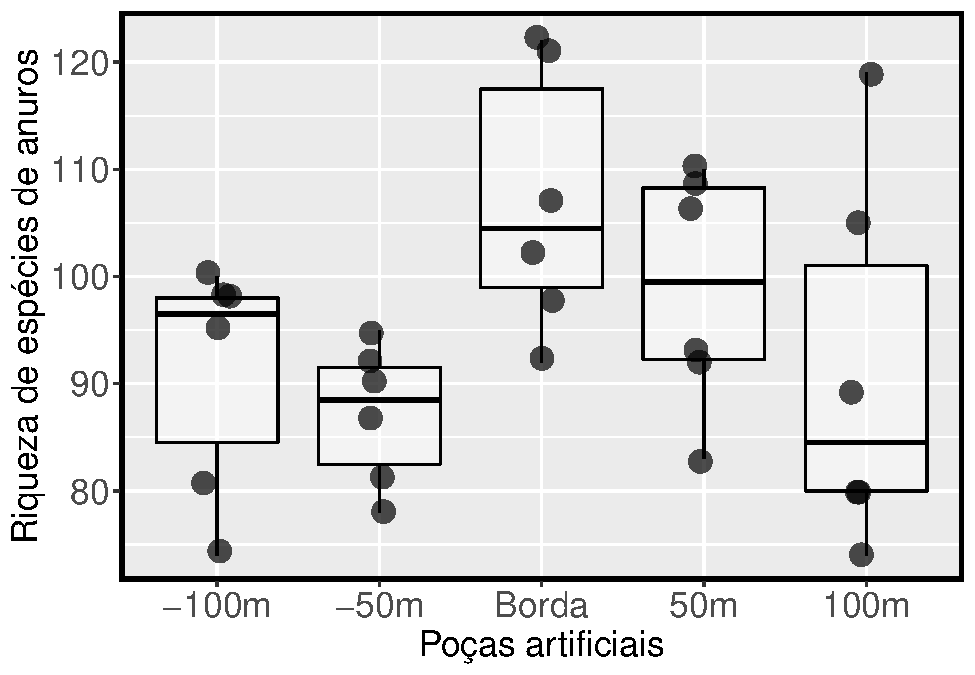
\includegraphics{livro_r_ecologia_files/figure-latex/unnamed-chunk-21-1.pdf}

\hypertarget{interpretauxe7uxe3o-dos-resultados}{%
\subsubsection{Interpretação dos resultados}\label{interpretauxe7uxe3o-dos-resultados}}

Com base no número de espécies raras (\emph{singletons} e \emph{doubletons}), o estimador Chao 1 indica a possibilidade de encontrarmos mais três espécies caso o esforço amostral fosse maior e não mostra tendência de estabilização da curva em uma assíntota.

\hypertarget{ace---abundance-based-coverage-estimador-chao-lee-1992-chao-et-al.-2000}{%
\subsection{\texorpdfstring{ACE - \emph{Abundance-based Coverage Estimador} (Chao \& Lee 1992, Chao et al.~2000):}{ACE - Abundance-based Coverage Estimador (Chao \& Lee 1992, Chao et al.~2000):}}\label{ace---abundance-based-coverage-estimador-chao-lee-1992-chao-et-al.-2000}}

Este método trabalha com a abundância das espécies raras (i.e.~abundância baixa). Entretanto, diferente do estimador anterior, esse método permite ao pesquisador determinar os limites para os quais uma espécie seja considerada rara. Em geral, são consideradas raras espécies com abundância entre 1 e 10 indivíduos. A riqueza estimada pode variar conforme se aumente ou diminua o limiar de abundância, e infelizmente não existem critérios biológicos definidos para a escolha do melhor intervalo.

\begin{quote}
\[ACE = S_{abund} + \frac{S_{rare}}{C_{ace}} + \frac{F_1}{C_{ace}}Y_{ace}^2\]
\end{quote}

onde:

\begin{quote}
\[Y_{ace}^2 = max \left[\frac{S_{rare}}{C_{ace}}\frac{\sum_{i=i}^{10}i(i-1)F1}{(N_{rare})({N_{rare} - 1)}}-1,0\right]\]
\end{quote}

\begin{quote}
\[C_{ace} = 1 - \frac{F1}{N_{rare}}\]
\end{quote}

\begin{quote}
\[N_{rare} = \sum_{i=1}^{10}iF_i\]
\end{quote}

Não precisa fazer cara feia, é óbvio que iremos usar o programa para fazer esses cálculos.

~

\hypertarget{exemplo-pruxe1tico---ace}{%
\subsubsection{Exemplo prático - ACE}\label{exemplo-pruxe1tico---ace}}

\hypertarget{explicauxe7uxe3o-dos-dados-1}{%
\paragraph{Explicação dos dados}\label{explicauxe7uxe3o-dos-dados-1}}

Usaremos os mesmos dados de 17 espécies de anuros amostradas em 14 dias de coletas de campo em um habitat reprodutivo localizado na região noroeste do estado de São Paulo, Brasil.

\textbf{Pergunta:}

\begin{quote}
Quantas espécies a mais poderiam ser amostradas caso aumentassemos o esforço amostral?
\end{quote}

\textbf{Predições}

\begin{quote}
\begin{itemize}
\tightlist
\item
  O número de espécies estimadas é similar ao número de espécies observada;
\item
  O número de espécies estimadas é maior do que o número de espécies observada.
\end{itemize}
\end{quote}

\textbf{Variáveis}

\begin{itemize}
\tightlist
\item
  Variáveis preditoras

  \begin{itemize}
  \tightlist
  \item
    matriz ou vetor com as abundâncias das espécies de anuros registradas em um habitat reprodutivo
  \end{itemize}
\end{itemize}

\textbf{Checklist}

\begin{itemize}
\tightlist
\item
  Verificar se a sua matriz está com as espécies nas colunas e as amostragens nas linhas
\item
  Verificar se os dados são de abundância e não presença e ausência
\end{itemize}

\hypertarget{anuxe1lise-1}{%
\subsection{Análise}\label{anuxe1lise-1}}

Calculo do estimador de riqueza - ACE

\begin{Shaded}
\begin{Highlighting}[]
\KeywordTok{library}\NormalTok{(vegan)}
\NormalTok{dados_coleta <-}\StringTok{ }\NormalTok{poca_anuros}
\NormalTok{est_ace <-}\StringTok{ }\KeywordTok{estaccumR}\NormalTok{(dados_coleta, }\DataTypeTok{permutations =} \DecValTok{100}\NormalTok{)}
\KeywordTok{summary}\NormalTok{(est_ace, }\DataTypeTok{display =} \StringTok{"ace"}\NormalTok{)}
\end{Highlighting}
\end{Shaded}

\begin{verbatim}
## $ace
##         N       ACE      2.5%    97.5%  Std.Dev
## Dia_9   1  7.420144  3.545190 13.71429 2.854333
## Dia_7   2 10.226919  6.146771 15.21781 2.551214
## Dia_12  3 11.618735  8.000000 17.11792 2.617299
## Dia_11  4 12.226959  8.475000 17.48784 2.490061
## Dia_3   5 13.114641  9.281723 20.04410 2.746716
## Dia_4   6 14.144536 10.000000 20.77212 2.847964
## Dia_6   7 15.259364 10.000000 21.70601 3.172167
## Dia_1   8 16.069255 11.000000 22.61582 3.410662
## Dia_10  9 17.730820 12.173645 24.75556 3.810667
## Dia_14 10 19.151979 13.430000 25.28994 4.098561
## Dia_2  11 20.709336 13.700889 25.72368 4.104579
## Dia_8  12 22.187560 16.144275 25.72368 3.525044
## Dia_13 13 23.622853 17.676471 25.72368 2.763304
## Dia_5  14 24.703704 24.703704 24.70370 0.000000
## 
## attr(,"class")
## [1] "summary.poolaccum"
\end{verbatim}

Visualizar os resultados com intervalo de confiança de 95\%

\begin{Shaded}
\begin{Highlighting}[]
\KeywordTok{library}\NormalTok{(ggplot2)}
\CommentTok{# preparando os dados para fazer o gráfico}
\NormalTok{resultados_ace <-}\StringTok{ }\KeywordTok{summary}\NormalTok{(est_ace, }\DataTypeTok{display =} \KeywordTok{c}\NormalTok{(}\StringTok{"S"}\NormalTok{, }\StringTok{"ace"}\NormalTok{))}
\NormalTok{res_ace <-}\StringTok{ }\KeywordTok{cbind}\NormalTok{(resultados_ace}\OperatorTok{$}\NormalTok{ace[,}\DecValTok{1}\OperatorTok{:}\DecValTok{4}\NormalTok{], resultados_ace}\OperatorTok{$}\NormalTok{S[,}\DecValTok{2}\OperatorTok{:}\DecValTok{4}\NormalTok{])}
\NormalTok{res_ace <-}\StringTok{ }\KeywordTok{as.data.frame}\NormalTok{(res_ace)}
\KeywordTok{colnames}\NormalTok{(res_ace) <-}\StringTok{ }\KeywordTok{c}\NormalTok{(}\StringTok{"Amostras"}\NormalTok{, }\StringTok{"ACE"}\NormalTok{, }\StringTok{"ACE_inferior"}\NormalTok{, }\StringTok{"ACE_superior"}\NormalTok{, }\StringTok{"Riqueza"}\NormalTok{,}
                        \StringTok{"R_inferior"}\NormalTok{, }\StringTok{"R_superior"}\NormalTok{)}

\CommentTok{# comando para o gráfico}
\KeywordTok{ggplot}\NormalTok{(res_ace, }\KeywordTok{aes}\NormalTok{(}\DataTypeTok{y =}\NormalTok{ Riqueza, }\DataTypeTok{x =}\NormalTok{ Amostras)) }\OperatorTok{+}
\StringTok{  }\KeywordTok{geom_point}\NormalTok{(}\KeywordTok{aes}\NormalTok{(}\DataTypeTok{y =}\NormalTok{ ACE, }\DataTypeTok{x =}\NormalTok{ Amostras }\OperatorTok{+}\StringTok{ }\FloatTok{0.1}\NormalTok{), }\DataTypeTok{size =} \DecValTok{5}\NormalTok{, }\DataTypeTok{color =} \StringTok{"blue"}\NormalTok{, }\DataTypeTok{alpha =} \DecValTok{1}\NormalTok{) }\OperatorTok{+}
\StringTok{  }\KeywordTok{geom_point}\NormalTok{(}\KeywordTok{aes}\NormalTok{(}\DataTypeTok{y =}\NormalTok{ Riqueza, }\DataTypeTok{x =}\NormalTok{ Amostras), }\DataTypeTok{size =} \DecValTok{5}\NormalTok{, }\DataTypeTok{color =} \StringTok{"red"}\NormalTok{, }\DataTypeTok{alpha =} \DecValTok{1}\NormalTok{) }\OperatorTok{+}
\StringTok{  }\KeywordTok{geom_line}\NormalTok{ (}\KeywordTok{aes}\NormalTok{(}\DataTypeTok{y =}\NormalTok{ ACE, }\DataTypeTok{x =}\NormalTok{ Amostras), }\DataTypeTok{color =} \StringTok{"blue"}\NormalTok{) }\OperatorTok{+}
\StringTok{  }\KeywordTok{geom_line}\NormalTok{ (}\KeywordTok{aes}\NormalTok{(}\DataTypeTok{y =}\NormalTok{ Riqueza, }\DataTypeTok{x =}\NormalTok{ Amostras), }\DataTypeTok{color =} \StringTok{"red"}\NormalTok{) }\OperatorTok{+}
\StringTok{  }\KeywordTok{geom_linerange}\NormalTok{(}\KeywordTok{aes}\NormalTok{(}\DataTypeTok{ymin =}\NormalTok{ ACE_inferior, }\DataTypeTok{ymax =}\NormalTok{ ACE_superior, }\DataTypeTok{x =}\NormalTok{ Amostras }\OperatorTok{+}\StringTok{ }\FloatTok{0.1}\NormalTok{),}
 \DataTypeTok{color =} \StringTok{"blue"}\NormalTok{) }\OperatorTok{+}
\StringTok{  }\KeywordTok{geom_linerange}\NormalTok{(}\KeywordTok{aes}\NormalTok{(}\DataTypeTok{ymin =}\NormalTok{ R_inferior, }\DataTypeTok{ymax =}\NormalTok{ R_superior, }\DataTypeTok{x =}\NormalTok{ Amostras), }\DataTypeTok{color =} \StringTok{"red"}\NormalTok{) }\OperatorTok{+}
\StringTok{  }\KeywordTok{ylab}\NormalTok{ (}\StringTok{"Estimador de riqueza - ACE"}\NormalTok{) }\OperatorTok{+}
\StringTok{  }\KeywordTok{xlab}\NormalTok{ (}\StringTok{"Número de amostras"}\NormalTok{) }\OperatorTok{+}
\StringTok{  }\KeywordTok{scale_x_continuous}\NormalTok{(}\DataTypeTok{limits =} \KeywordTok{c}\NormalTok{(}\DecValTok{1}\NormalTok{,}\DecValTok{15}\NormalTok{), }\DataTypeTok{breaks=}\KeywordTok{seq}\NormalTok{(}\DecValTok{1}\NormalTok{,}\DecValTok{15}\NormalTok{,}\DecValTok{1}\NormalTok{)) }\OperatorTok{+}
\StringTok{  }\KeywordTok{geom_point}\NormalTok{(}\DataTypeTok{y=} \FloatTok{7.5}\NormalTok{, }\DataTypeTok{x =} \DecValTok{9}\NormalTok{, }\DataTypeTok{size =} \DecValTok{5}\NormalTok{, }\DataTypeTok{color =} \StringTok{"blue"}\NormalTok{, }\DataTypeTok{alpha =} \DecValTok{1}\NormalTok{) }\OperatorTok{+}\StringTok{ }
\StringTok{  }\KeywordTok{geom_point}\NormalTok{(}\DataTypeTok{y=} \FloatTok{5.9}\NormalTok{, }\DataTypeTok{x =} \DecValTok{9}\NormalTok{, }\DataTypeTok{size =} \DecValTok{5}\NormalTok{, }\DataTypeTok{color =} \StringTok{"red"}\NormalTok{, }\DataTypeTok{alpha =} \DecValTok{1}\NormalTok{) }\OperatorTok{+}\StringTok{ }
\StringTok{  }\KeywordTok{geom_label}\NormalTok{( }\DataTypeTok{y =} \FloatTok{7.5}\NormalTok{, }\DataTypeTok{x =} \FloatTok{11.7}\NormalTok{, }\DataTypeTok{label =} \StringTok{"Riqueza estimada - ACE"}\NormalTok{) }\OperatorTok{+}
\StringTok{  }\KeywordTok{geom_label}\NormalTok{( }\DataTypeTok{y =} \FloatTok{5.9}\NormalTok{, }\DataTypeTok{x =} \FloatTok{11.3}\NormalTok{, }\DataTypeTok{label =} \StringTok{"Riqueza observada"}\NormalTok{)}
\end{Highlighting}
\end{Shaded}

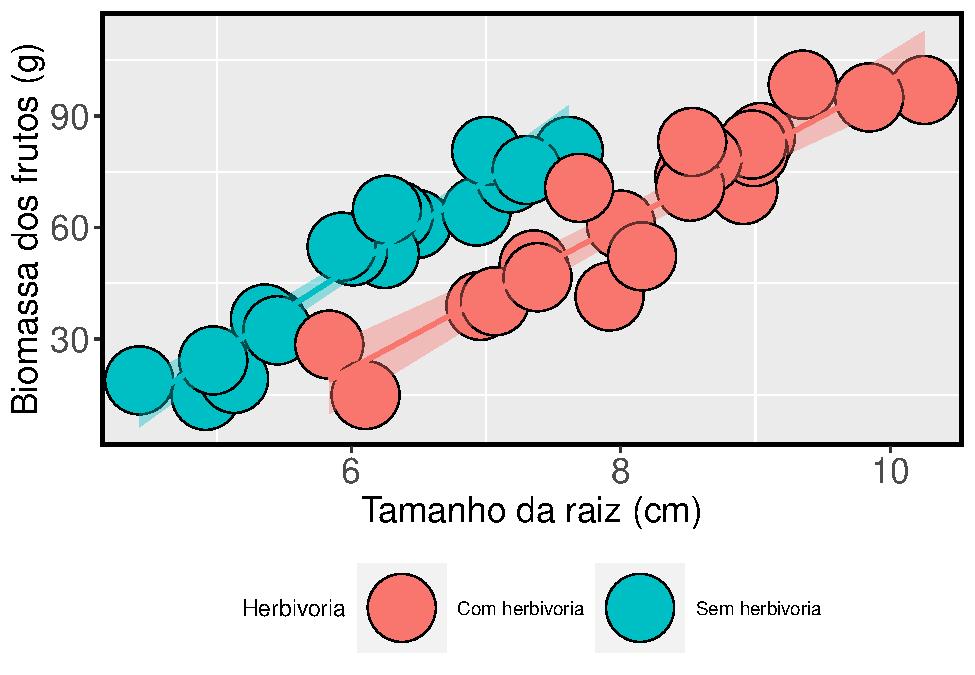
\includegraphics{livro_r_ecologia_files/figure-latex/unnamed-chunk-23-1.pdf}

\hypertarget{interpretauxe7uxe3o-dos-resultados-1}{%
\subsubsection{Interpretação dos resultados}\label{interpretauxe7uxe3o-dos-resultados-1}}

Com base no número de espécies raras (abundância menor que 10 indivíduos - \emph{default}), o estimador ACE indica a possibilidade de encontrarmos mais sete espécies caso o esforço amostral fosse maior e não mostrou tendência de estabilição da curva em uma assíntota.

\hypertarget{estimadores-baseados-na-inciduxeancia-das-espuxe9cies}{%
\section{Estimadores baseados na incidência das espécies}\label{estimadores-baseados-na-inciduxeancia-das-espuxe9cies}}

\hypertarget{chao-2---chao-1987}{%
\subsection{CHAO 2 - (Chao 1987):}\label{chao-2---chao-1987}}

De acordo com Anne Chao, o estimador Chao 1 pode ser modificado para uso com dados de presença/ausência levando em conta a distribuição das espécies entre amostras. Neste caso é
necessário conhecer o número de espécies encontradas em somente uma amostra e o
número de espécies encontradas exatamente em duas amostras. Essa variação ficou denominada como
Chao 2:

\begin{quote}
\[Chao_{2} = S_{obs} + \left(\frac{m-1}{m}\right)\left(\frac{Q_1(Q_1-1)}{2(Q_2 + 1}\right)\]
\end{quote}

onde:

\begin{itemize}
\item
  Sobs = o número de espécies na comunidade,
\item
  \emph{m} = número de amostragens,
\item
  Q1 = número de espécies observadas em uma amostragem (espécies \emph{uniques}),
\item
  Q2 = número de espécies observadas em duas amostragens (espécies \emph{duplicates}).
\end{itemize}

O valor de Chao2 é máximo quando as espécies menos uma são únicas (\emph{uniques}). Neste caso, a riqueza estimada é aproximadamente o dobro da riqueza observada. Colwell \& Coddington (1994) encontraram que o valor de Chao 2 mostrou ser o estimador menos enviesado para amostras com tamanho pequeno.

~

\hypertarget{exemplo-pruxe1tico---chao-2}{%
\subsubsection{Exemplo prático - Chao 2}\label{exemplo-pruxe1tico---chao-2}}

\hypertarget{explicauxe7uxe3o-dos-dados-2}{%
\paragraph{Explicação dos dados}\label{explicauxe7uxe3o-dos-dados-2}}

Usaremos os mesmos dados de 17 espécies de anuros amostradas em 14 dias de coletas de campo em um habitat reprodutivo localizado na região noroeste do estado de São Paulo, Brasil.

\textbf{Pergunta:}

\begin{quote}
Quantas espécies a mais poderiam ser amostradas caso aumentassemos o esforço amostral?
\end{quote}

\textbf{Predições}

\begin{quote}
\begin{itemize}
\tightlist
\item
  O número de espécies estimadas é similar ao número de espécies observada;
\item
  O número de espécies estimadas é maior do que o número de espécies observada.
\end{itemize}
\end{quote}

\textbf{Variáveis}

\begin{itemize}
\tightlist
\item
  Variáveis preditoras

  \begin{itemize}
  \tightlist
  \item
    matriz ou vetor com a incidência das espécies de anuros registradas em um habitat reprodutivo
  \end{itemize}
\end{itemize}

\textbf{Checklist}

\begin{itemize}
\tightlist
\item
  Verificar se a sua matriz está com as espécies nas colunas e as amostragens nas linhas
\end{itemize}

\hypertarget{anuxe1lise-2}{%
\subsection{Análise}\label{anuxe1lise-2}}

Calculo do estimador de riqueza - Chao 2

\begin{Shaded}
\begin{Highlighting}[]
\KeywordTok{library}\NormalTok{(vegan)}
\NormalTok{dados_coleta <-}\StringTok{ }\NormalTok{poca_anuros}
\NormalTok{est_chao2 <-}\StringTok{ }\KeywordTok{poolaccum}\NormalTok{(dados_coleta, }\DataTypeTok{permutations =} \DecValTok{100}\NormalTok{)}
\KeywordTok{summary}\NormalTok{(est_chao2, }\DataTypeTok{display =} \StringTok{"chao"}\NormalTok{)}
\end{Highlighting}
\end{Shaded}

\begin{verbatim}
## $chao
##        N     Chao      2.5%    97.5%  Std.Dev
##  [1,]  3 13.71862  8.060833 21.47292 3.956134
##  [2,]  4 15.73406  9.500000 30.07812 5.849969
##  [3,]  5 17.00113 10.432500 33.65000 6.015478
##  [4,]  6 18.16826 10.891667 32.98125 6.139506
##  [5,]  7 19.33200 11.992857 37.00000 6.650056
##  [6,]  8 20.80996 12.218750 35.98281 6.549691
##  [7,]  9 23.60704 12.183333 40.41111 7.581342
##  [8,] 10 25.05525 14.327500 42.20000 7.502622
##  [9,] 11 26.83591 14.818182 42.45455 7.098248
## [10,] 12 28.76917 21.333333 39.45833 6.131360
## [11,] 13 30.75615 22.384615 39.61538 5.320240
## [12,] 14 33.71429 33.714286 33.71429 0.000000
## 
## attr(,"class")
## [1] "summary.poolaccum"
\end{verbatim}

Visualizar os resultados com intervalo de confiança de 95\%

\begin{Shaded}
\begin{Highlighting}[]
\KeywordTok{library}\NormalTok{(ggplot2)}
\CommentTok{# preparando os dados para fazer o gráfico}
\NormalTok{resultados_chao2 <-}\StringTok{ }\KeywordTok{summary}\NormalTok{(est_chao2, }\DataTypeTok{display =} \KeywordTok{c}\NormalTok{(}\StringTok{"S"}\NormalTok{, }\StringTok{"chao"}\NormalTok{))}
\NormalTok{res_chao2 <-}\StringTok{ }\KeywordTok{cbind}\NormalTok{(resultados_chao2}\OperatorTok{$}\NormalTok{chao[,}\DecValTok{1}\OperatorTok{:}\DecValTok{4}\NormalTok{], resultados_chao2}\OperatorTok{$}\NormalTok{S[,}\DecValTok{2}\OperatorTok{:}\DecValTok{4}\NormalTok{])}
\NormalTok{res_chao2 <-}\StringTok{ }\KeywordTok{as.data.frame}\NormalTok{(res_chao2)}
\KeywordTok{colnames}\NormalTok{(res_chao2) <-}\StringTok{ }\KeywordTok{c}\NormalTok{(}\StringTok{"Amostras"}\NormalTok{, }\StringTok{"Chao2"}\NormalTok{, }\StringTok{"C_inferior"}\NormalTok{, }\StringTok{"C_superior"}\NormalTok{, }\StringTok{"Riqueza"}\NormalTok{,}
                        \StringTok{"R_inferior"}\NormalTok{, }\StringTok{"R_superior"}\NormalTok{)}

\CommentTok{# comando para o gráfico}
\KeywordTok{ggplot}\NormalTok{(res_chao2, }\KeywordTok{aes}\NormalTok{(}\DataTypeTok{y =}\NormalTok{ Riqueza, }\DataTypeTok{x =}\NormalTok{ Amostras)) }\OperatorTok{+}
\StringTok{  }\KeywordTok{geom_point}\NormalTok{(}\KeywordTok{aes}\NormalTok{(}\DataTypeTok{y =}\NormalTok{ Chao2, }\DataTypeTok{x =}\NormalTok{ Amostras }\OperatorTok{+}\StringTok{ }\FloatTok{0.1}\NormalTok{), }\DataTypeTok{size =} \DecValTok{5}\NormalTok{, }\DataTypeTok{color =} \StringTok{"blue"}\NormalTok{, }\DataTypeTok{alpha =} \DecValTok{1}\NormalTok{) }\OperatorTok{+}
\StringTok{  }\KeywordTok{geom_point}\NormalTok{(}\KeywordTok{aes}\NormalTok{(}\DataTypeTok{y =}\NormalTok{ Riqueza, }\DataTypeTok{x =}\NormalTok{ Amostras), }\DataTypeTok{size =} \DecValTok{5}\NormalTok{, }\DataTypeTok{color =} \StringTok{"red"}\NormalTok{, }\DataTypeTok{alpha =} \DecValTok{1}\NormalTok{) }\OperatorTok{+}
\StringTok{  }\KeywordTok{geom_line}\NormalTok{ (}\KeywordTok{aes}\NormalTok{(}\DataTypeTok{y =}\NormalTok{ Chao2, }\DataTypeTok{x =}\NormalTok{ Amostras), }\DataTypeTok{color =} \StringTok{"blue"}\NormalTok{) }\OperatorTok{+}
\StringTok{  }\KeywordTok{geom_line}\NormalTok{ (}\KeywordTok{aes}\NormalTok{(}\DataTypeTok{y =}\NormalTok{ Riqueza, }\DataTypeTok{x =}\NormalTok{ Amostras), }\DataTypeTok{color =} \StringTok{"red"}\NormalTok{) }\OperatorTok{+}
\StringTok{  }\KeywordTok{geom_linerange}\NormalTok{(}\KeywordTok{aes}\NormalTok{(}\DataTypeTok{ymin =}\NormalTok{ C_inferior, }\DataTypeTok{ymax =}\NormalTok{ C_superior, }\DataTypeTok{x =}\NormalTok{ Amostras }\OperatorTok{+}\StringTok{ }\FloatTok{0.1}\NormalTok{),}
 \DataTypeTok{color =} \StringTok{"blue"}\NormalTok{) }\OperatorTok{+}
\StringTok{  }\KeywordTok{geom_linerange}\NormalTok{(}\KeywordTok{aes}\NormalTok{(}\DataTypeTok{ymin =}\NormalTok{ R_inferior, }\DataTypeTok{ymax =}\NormalTok{ R_superior, }\DataTypeTok{x =}\NormalTok{ Amostras), }\DataTypeTok{color =} \StringTok{"red"}\NormalTok{) }\OperatorTok{+}
\StringTok{  }\KeywordTok{ylab}\NormalTok{ (}\StringTok{"Estimador de riqueza - Chao 2"}\NormalTok{) }\OperatorTok{+}
\StringTok{  }\KeywordTok{xlab}\NormalTok{ (}\StringTok{"Número de amostras"}\NormalTok{) }\OperatorTok{+}
\StringTok{  }\KeywordTok{scale_x_continuous}\NormalTok{(}\DataTypeTok{limits =} \KeywordTok{c}\NormalTok{(}\DecValTok{1}\NormalTok{,}\DecValTok{15}\NormalTok{), }\DataTypeTok{breaks=}\KeywordTok{seq}\NormalTok{(}\DecValTok{1}\NormalTok{,}\DecValTok{15}\NormalTok{,}\DecValTok{1}\NormalTok{)) }\OperatorTok{+}
\StringTok{  }\KeywordTok{geom_point}\NormalTok{(}\DataTypeTok{y=} \FloatTok{9.8}\NormalTok{, }\DataTypeTok{x =} \DecValTok{10}\NormalTok{, }\DataTypeTok{size =} \DecValTok{5}\NormalTok{, }\DataTypeTok{color =} \StringTok{"blue"}\NormalTok{, }\DataTypeTok{alpha =} \DecValTok{1}\NormalTok{) }\OperatorTok{+}\StringTok{ }
\StringTok{  }\KeywordTok{geom_point}\NormalTok{(}\DataTypeTok{y=} \FloatTok{7.7}\NormalTok{, }\DataTypeTok{x =} \DecValTok{10}\NormalTok{, }\DataTypeTok{size =} \DecValTok{5}\NormalTok{, }\DataTypeTok{color =} \StringTok{"red"}\NormalTok{, }\DataTypeTok{alpha =} \DecValTok{1}\NormalTok{) }\OperatorTok{+}\StringTok{ }
\StringTok{  }\KeywordTok{geom_label}\NormalTok{( }\DataTypeTok{y =} \FloatTok{9.8}\NormalTok{, }\DataTypeTok{x =} \FloatTok{12.95}\NormalTok{, }\DataTypeTok{label =} \StringTok{"Riqueza estimada - Chao 2"}\NormalTok{) }\OperatorTok{+}
\StringTok{  }\KeywordTok{geom_label}\NormalTok{( }\DataTypeTok{y =} \FloatTok{7.7}\NormalTok{, }\DataTypeTok{x =} \FloatTok{12.3}\NormalTok{, }\DataTypeTok{label =} \StringTok{"Riqueza observada"}\NormalTok{)}
\end{Highlighting}
\end{Shaded}

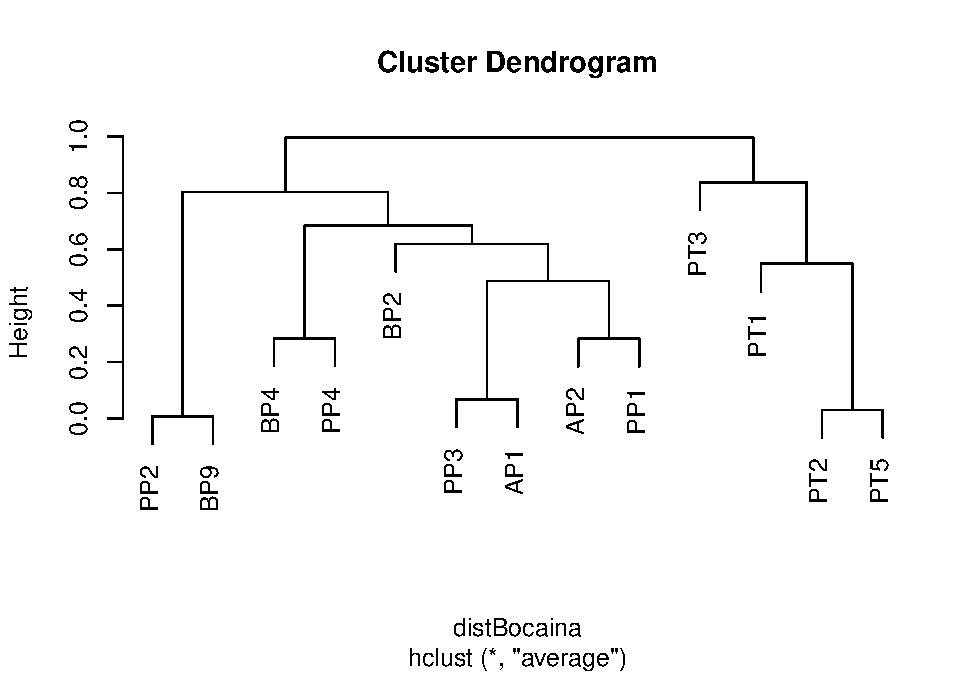
\includegraphics{livro_r_ecologia_files/figure-latex/unnamed-chunk-25-1.pdf}

\hypertarget{interpretauxe7uxe3o-dos-resultados-2}{%
\subsubsection{Interpretação dos resultados}\label{interpretauxe7uxe3o-dos-resultados-2}}

Com base no número de espécies raras (\emph{uniques} e \emph{duplicates}), Chao 2 estimou a possibilidade de encontrarmos mais dezesseis espécies caso o esforço amostral fosse maior e não mostrou tendência de estabilização da curva em uma assíntota.

\hypertarget{jackknife-1-burnham-overton-1978-1979}{%
\subsection{JACKKNIFE 1 (Burnham \& Overton 1978, 1979):}\label{jackknife-1-burnham-overton-1978-1979}}

Este estimador baseia-se no número de espécies que ocorrem em somente uma amostra (Q1).

\begin{quote}
\[S_{jack1} = S_{obs} + Q1\left(\frac{m - 1}{m}\right)\]
\end{quote}

onde:

\begin{itemize}
\item
  Sobs = o número de espécies na comunidade,
\item
  Q1 = número de espécies observadas em uma amostragem (espécies \emph{uniques}),
\item
  \emph{m} = número de amostragens.
\end{itemize}

Palmer (1990) verificou que Jackknife 1 foi o estimador mais preciso e menos enviesado comparado a outros métodos de extrapolação.

~

\hypertarget{exemplo-pruxe1tico---jackknife-1}{%
\subsubsection{Exemplo prático - Jackknife 1}\label{exemplo-pruxe1tico---jackknife-1}}

\hypertarget{explicauxe7uxe3o-dos-dados-3}{%
\paragraph{Explicação dos dados}\label{explicauxe7uxe3o-dos-dados-3}}

Usaremos os mesmos dados de 17 espécies de anuros amostradas em 14 dias de coletas de campo em um habitat reprodutivo localizado na região noroeste do estado de São Paulo, Brasil.

\textbf{Pergunta:}

\begin{quote}
Quantas espécies a mais poderiam ser amostradas caso aumentassemos o esforço amostral?
\end{quote}

\textbf{Predições}

\begin{quote}
\begin{itemize}
\tightlist
\item
  O número de espécies estimadas é similar ao número de espécies observada;
\item
  O número de espécies estimadas é maior do que o número de espécies observada.
\end{itemize}
\end{quote}

\textbf{Variáveis}

\begin{itemize}
\tightlist
\item
  Variáveis preditoras

  \begin{itemize}
  \tightlist
  \item
    matriz ou vetor com as abundâncias das espécies de anuros registradas em um habitat reprodutivo
  \end{itemize}
\end{itemize}

\textbf{Checklist}

\begin{itemize}
\tightlist
\item
  Verificar se a sua matriz está com as espécies nas colunas e as amostragens nas linhas
\end{itemize}

\hypertarget{anuxe1lise-3}{%
\subsection{Análise}\label{anuxe1lise-3}}

Calculo do estimador de riqueza - Jackknife 1

\begin{Shaded}
\begin{Highlighting}[]
\KeywordTok{library}\NormalTok{(vegan)}
\NormalTok{dados_coleta <-}\StringTok{ }\NormalTok{poca_anuros}
\NormalTok{est_jack1 <-}\StringTok{ }\KeywordTok{poolaccum}\NormalTok{(dados_coleta, }\DataTypeTok{permutations =} \DecValTok{100}\NormalTok{)}
\KeywordTok{summary}\NormalTok{(est_jack1, }\DataTypeTok{display =} \StringTok{"jack1"}\NormalTok{)}
\end{Highlighting}
\end{Shaded}

\begin{verbatim}
## $jack1
##        N Jackknife 1      2.5%    97.5%  Std.Dev
##  [1,]  3    14.08667  8.650000 19.33333 2.712824
##  [2,]  4    14.98250  9.750000 21.16875 2.942259
##  [3,]  5    15.76600  9.800000 21.12500 2.795097
##  [4,]  6    16.56833  9.833333 23.19167 2.878779
##  [5,]  7    17.61143 12.782143 23.04286 2.898267
##  [6,]  8    18.32625 13.750000 24.00000 2.799198
##  [7,]  9    19.14667 14.200000 24.11111 2.659028
##  [8,] 10    19.63300 14.800000 23.77250 2.469288
##  [9,] 11    20.54455 16.727273 23.84091 2.068914
## [10,] 12    21.23417 18.141667 23.41667 1.861947
## [11,] 13    21.71692 18.692308 23.46154 1.503642
## [12,] 14    22.57143 22.571429 22.57143 0.000000
## 
## attr(,"class")
## [1] "summary.poolaccum"
\end{verbatim}

Visualizar os resultados com 95\% intervalo de confiança

\begin{Shaded}
\begin{Highlighting}[]
\KeywordTok{library}\NormalTok{(ggplot2)}
\CommentTok{# preparando os dados para fazer o gráfico}
\NormalTok{resultados_jack1 <-}\StringTok{ }\KeywordTok{summary}\NormalTok{(est_jack1, }\DataTypeTok{display =} \KeywordTok{c}\NormalTok{(}\StringTok{"S"}\NormalTok{, }\StringTok{"jack1"}\NormalTok{))}
\NormalTok{res_jack1 <-}\StringTok{ }\KeywordTok{cbind}\NormalTok{(resultados_jack1}\OperatorTok{$}\NormalTok{jack1[,}\DecValTok{1}\OperatorTok{:}\DecValTok{4}\NormalTok{], resultados_jack1}\OperatorTok{$}\NormalTok{S[,}\DecValTok{2}\OperatorTok{:}\DecValTok{4}\NormalTok{])}
\NormalTok{res_jack1 <-}\StringTok{ }\KeywordTok{as.data.frame}\NormalTok{(res_jack1)}
\KeywordTok{colnames}\NormalTok{(res_jack1) <-}\StringTok{ }\KeywordTok{c}\NormalTok{(}\StringTok{"Amostras"}\NormalTok{, }\StringTok{"JACK1"}\NormalTok{, }\StringTok{"JACK1_inferior"}\NormalTok{, }\StringTok{"JACK1_superior"}\NormalTok{, }\StringTok{"Riqueza"}\NormalTok{,}
                        \StringTok{"R_inferior"}\NormalTok{, }\StringTok{"R_superior"}\NormalTok{)}

\CommentTok{# comando para o gráfico}
\KeywordTok{ggplot}\NormalTok{(res_jack1, }\KeywordTok{aes}\NormalTok{(}\DataTypeTok{y =}\NormalTok{ Riqueza, }\DataTypeTok{x =}\NormalTok{ Amostras)) }\OperatorTok{+}
\StringTok{  }\KeywordTok{geom_point}\NormalTok{(}\KeywordTok{aes}\NormalTok{(}\DataTypeTok{y =}\NormalTok{ JACK1, }\DataTypeTok{x =}\NormalTok{ Amostras }\OperatorTok{+}\StringTok{ }\FloatTok{0.1}\NormalTok{), }\DataTypeTok{size =} \DecValTok{5}\NormalTok{, }\DataTypeTok{color =} \StringTok{"blue"}\NormalTok{, }\DataTypeTok{alpha =} \DecValTok{1}\NormalTok{) }\OperatorTok{+}
\StringTok{  }\KeywordTok{geom_point}\NormalTok{(}\KeywordTok{aes}\NormalTok{(}\DataTypeTok{y =}\NormalTok{ Riqueza, }\DataTypeTok{x =}\NormalTok{ Amostras), }\DataTypeTok{size =} \DecValTok{5}\NormalTok{, }\DataTypeTok{color =} \StringTok{"red"}\NormalTok{, }\DataTypeTok{alpha =} \DecValTok{1}\NormalTok{) }\OperatorTok{+}
\StringTok{  }\KeywordTok{geom_line}\NormalTok{ (}\KeywordTok{aes}\NormalTok{(}\DataTypeTok{y =}\NormalTok{ JACK1, }\DataTypeTok{x =}\NormalTok{ Amostras), }\DataTypeTok{color =} \StringTok{"blue"}\NormalTok{) }\OperatorTok{+}
\StringTok{  }\KeywordTok{geom_line}\NormalTok{ (}\KeywordTok{aes}\NormalTok{(}\DataTypeTok{y =}\NormalTok{ Riqueza, }\DataTypeTok{x =}\NormalTok{ Amostras), }\DataTypeTok{color =} \StringTok{"red"}\NormalTok{) }\OperatorTok{+}
\StringTok{  }\KeywordTok{geom_linerange}\NormalTok{(}\KeywordTok{aes}\NormalTok{(}\DataTypeTok{ymin =}\NormalTok{ JACK1_inferior, }\DataTypeTok{ymax =}\NormalTok{ JACK1_superior, }\DataTypeTok{x =}\NormalTok{ Amostras }\OperatorTok{+}\StringTok{ }\FloatTok{0.1}\NormalTok{),}
 \DataTypeTok{color =} \StringTok{"blue"}\NormalTok{) }\OperatorTok{+}
\StringTok{  }\KeywordTok{geom_linerange}\NormalTok{(}\KeywordTok{aes}\NormalTok{(}\DataTypeTok{ymin =}\NormalTok{ R_inferior, }\DataTypeTok{ymax =}\NormalTok{ R_superior, }\DataTypeTok{x =}\NormalTok{ Amostras), }\DataTypeTok{color =} \StringTok{"red"}\NormalTok{) }\OperatorTok{+}
\StringTok{  }\KeywordTok{ylab}\NormalTok{ (}\StringTok{"Estimador de riqueza - Jackknife 1"}\NormalTok{) }\OperatorTok{+}
\StringTok{  }\KeywordTok{xlab}\NormalTok{ (}\StringTok{"Número de amostras"}\NormalTok{) }\OperatorTok{+}
\StringTok{  }\KeywordTok{scale_x_continuous}\NormalTok{(}\DataTypeTok{limits =} \KeywordTok{c}\NormalTok{(}\DecValTok{1}\NormalTok{,}\DecValTok{15}\NormalTok{), }\DataTypeTok{breaks=}\KeywordTok{seq}\NormalTok{(}\DecValTok{1}\NormalTok{,}\DecValTok{15}\NormalTok{,}\DecValTok{1}\NormalTok{)) }\OperatorTok{+}
\StringTok{  }\KeywordTok{geom_point}\NormalTok{(}\DataTypeTok{y=} \FloatTok{9.9}\NormalTok{, }\DataTypeTok{x =} \DecValTok{9}\NormalTok{, }\DataTypeTok{size =} \DecValTok{5}\NormalTok{, }\DataTypeTok{color =} \StringTok{"blue"}\NormalTok{, }\DataTypeTok{alpha =} \DecValTok{1}\NormalTok{) }\OperatorTok{+}\StringTok{ }
\StringTok{  }\KeywordTok{geom_point}\NormalTok{(}\DataTypeTok{y=} \FloatTok{8.6}\NormalTok{, }\DataTypeTok{x =} \DecValTok{9}\NormalTok{, }\DataTypeTok{size =} \DecValTok{5}\NormalTok{, }\DataTypeTok{color =} \StringTok{"red"}\NormalTok{, }\DataTypeTok{alpha =} \DecValTok{1}\NormalTok{) }\OperatorTok{+}\StringTok{ }
\StringTok{  }\KeywordTok{geom_label}\NormalTok{( }\DataTypeTok{y =} \FloatTok{9.9}\NormalTok{, }\DataTypeTok{x =} \FloatTok{12.5}\NormalTok{, }\DataTypeTok{label =} \StringTok{"Riqueza estimada - Jackknife 1"}\NormalTok{) }\OperatorTok{+}
\StringTok{  }\KeywordTok{geom_label}\NormalTok{( }\DataTypeTok{y =} \FloatTok{8.6}\NormalTok{, }\DataTypeTok{x =} \FloatTok{11.5}\NormalTok{, }\DataTypeTok{label =} \StringTok{"Riqueza observada"}\NormalTok{)}
\end{Highlighting}
\end{Shaded}

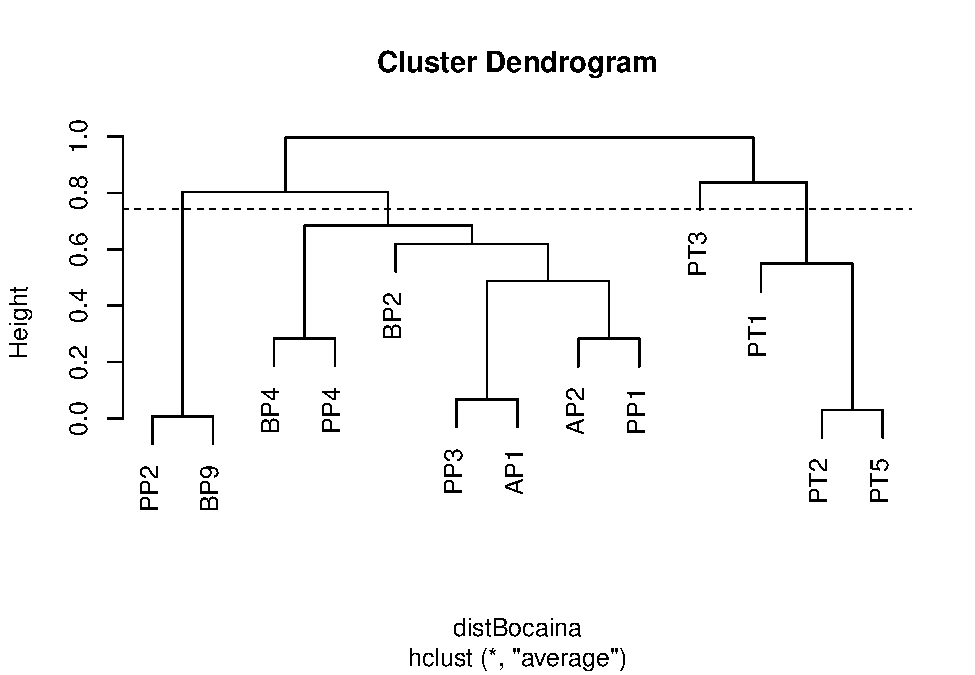
\includegraphics{livro_r_ecologia_files/figure-latex/unnamed-chunk-27-1.pdf}

\hypertarget{interpretauxe7uxe3o-dos-resultados-3}{%
\subsubsection{Interpretação dos resultados}\label{interpretauxe7uxe3o-dos-resultados-3}}

Com base no número de espécies raras, o estimador Jackknife 1 calculou a possibilidade de encontrarmos mais seis espécies caso o esforço amostral fosse maior e não mostrou tendência de estabilização da curva em uma assíntota.

\hypertarget{jackknife-2-burnham-overton-1978-1979-palmer-1991}{%
\subsection{JACKKNIFE 2 (Burnham \& Overton 1978, 1979, Palmer 1991):}\label{jackknife-2-burnham-overton-1978-1979-palmer-1991}}

Este método basea-se no número de espécies que ocorrem em apenas uma amostra e no número de espécies que ocorrem em exatamente duas amostras.

\begin{quote}
\[S_{jack2} = S_{obs} + \left[\frac{Q_1(2m - 3)}{m}-\frac{Q_2(m - 2)^2}{m(m-1)}\right]\]
\end{quote}

onde:

\begin{itemize}
\item
  Sobs = o número de espécies na comunidade,
\item
  \emph{m} = número de amostragens,
\item
  Q1 = número de espécies observadas em uma amostragem (espécies \emph{uniques}),
\item
  Q2 = número de espécies observadas em duas amostragens (espécies \emph{duplicates}).
\end{itemize}

~

\hypertarget{exemplo-pruxe1tico---jackknife-2}{%
\subsubsection{Exemplo prático - Jackknife 2}\label{exemplo-pruxe1tico---jackknife-2}}

\hypertarget{explicauxe7uxe3o-dos-dados-4}{%
\paragraph{Explicação dos dados}\label{explicauxe7uxe3o-dos-dados-4}}

Usaremos os mesmos dados de 17 espécies de anuros amostradas em 14 dias de coletas de campo em um habitat reprodutivo localizado na região noroeste do estado de São Paulo, Brasil.

\textbf{Pergunta:}

\begin{quote}
Quantas espécies a mais poderiam ser amostradas caso aumentassemos o esforço amostral?
\end{quote}

\textbf{Predições}

\begin{quote}
\begin{itemize}
\tightlist
\item
  O número de espécies estimadas é similar ao número de espécies observada;
\item
  O número de espécies estimadas é maior do que o número de espécies observada.
\end{itemize}
\end{quote}

\textbf{Variáveis}

\begin{itemize}
\tightlist
\item
  Variáveis preditoras

  \begin{itemize}
  \tightlist
  \item
    matriz ou vetor com as abundâncias das espécies de anuros registradas em um habitat reprodutivo
  \end{itemize}
\end{itemize}

\textbf{Checklist}

\begin{itemize}
\tightlist
\item
  Verificar se a sua matriz está com as espécies nas colunas e as amostragens nas linhas
\end{itemize}

\hypertarget{anuxe1lise-4}{%
\subsection{Análise}\label{anuxe1lise-4}}

Calculo do estimador de riqueza - Jackknife 2

\begin{Shaded}
\begin{Highlighting}[]
\KeywordTok{library}\NormalTok{(vegan)}
\NormalTok{dados_coleta <-}\StringTok{ }\NormalTok{poca_anuros}
\NormalTok{est_jack2 <-}\StringTok{ }\KeywordTok{poolaccum}\NormalTok{(dados_coleta, }\DataTypeTok{permutations =} \DecValTok{100}\NormalTok{)}
\KeywordTok{summary}\NormalTok{(est_jack2, }\DataTypeTok{display =} \StringTok{"jack2"}\NormalTok{)}
\end{Highlighting}
\end{Shaded}

\begin{verbatim}
## $jack2
##        N Jackknife 2      2.5%    97.5%  Std.Dev
##  [1,]  3    14.43667  6.966667 21.58750 3.192723
##  [2,]  4    15.72000 10.833333 22.04375 3.368783
##  [3,]  5    16.65450  9.762500 24.63875 3.967087
##  [4,]  6    18.22933 11.620000 25.21167 4.066554
##  [5,]  7    19.60929 12.952381 27.21250 4.174452
##  [6,]  8    20.72964 12.941518 27.56250 4.166807
##  [7,]  9    21.81514 14.636806 27.98611 3.937369
##  [8,] 10    22.86289 16.359167 29.45472 3.619994
##  [9,] 11    24.20527 17.570682 28.35455 3.312617
## [10,] 12    25.17462 20.242424 28.49242 2.800070
## [11,] 13    26.18673 21.301282 28.60897 1.769616
## [12,] 14    26.92308 26.923077 26.92308 0.000000
## 
## attr(,"class")
## [1] "summary.poolaccum"
\end{verbatim}

Visualizar os resultados com intervalo de confiança de 95\%

\begin{Shaded}
\begin{Highlighting}[]
\KeywordTok{library}\NormalTok{(ggplot2)}
\CommentTok{# preparando os dados para fazer o gráfico}
\NormalTok{resultados_jack2 <-}\StringTok{ }\KeywordTok{summary}\NormalTok{(est_jack2, }\DataTypeTok{display =} \KeywordTok{c}\NormalTok{(}\StringTok{"S"}\NormalTok{, }\StringTok{"jack2"}\NormalTok{))}
\NormalTok{res_jack2 <-}\StringTok{ }\KeywordTok{cbind}\NormalTok{(resultados_jack2}\OperatorTok{$}\NormalTok{jack2[,}\DecValTok{1}\OperatorTok{:}\DecValTok{4}\NormalTok{], resultados_jack2}\OperatorTok{$}\NormalTok{S[,}\DecValTok{2}\OperatorTok{:}\DecValTok{4}\NormalTok{])}
\NormalTok{res_jack2 <-}\StringTok{ }\KeywordTok{as.data.frame}\NormalTok{(res_jack2)}
\KeywordTok{colnames}\NormalTok{(res_jack2) <-}\StringTok{ }\KeywordTok{c}\NormalTok{(}\StringTok{"Amostras"}\NormalTok{, }\StringTok{"JACK2"}\NormalTok{, }\StringTok{"JACK2_inferior"}\NormalTok{, }\StringTok{"JACK2_superior"}\NormalTok{, }\StringTok{"Riqueza"}\NormalTok{,}
                        \StringTok{"R_inferior"}\NormalTok{, }\StringTok{"R_superior"}\NormalTok{)}

\CommentTok{# comando para o gráfico}
\KeywordTok{ggplot}\NormalTok{(res_jack2, }\KeywordTok{aes}\NormalTok{(}\DataTypeTok{y =}\NormalTok{ Riqueza, }\DataTypeTok{x =}\NormalTok{ Amostras)) }\OperatorTok{+}
\StringTok{  }\KeywordTok{geom_point}\NormalTok{(}\KeywordTok{aes}\NormalTok{(}\DataTypeTok{y =}\NormalTok{ JACK2, }\DataTypeTok{x =}\NormalTok{ Amostras }\OperatorTok{+}\StringTok{ }\FloatTok{0.1}\NormalTok{), }\DataTypeTok{size =} \DecValTok{5}\NormalTok{, }\DataTypeTok{color =} \StringTok{"blue"}\NormalTok{, }\DataTypeTok{alpha =} \DecValTok{1}\NormalTok{) }\OperatorTok{+}
\StringTok{  }\KeywordTok{geom_point}\NormalTok{(}\KeywordTok{aes}\NormalTok{(}\DataTypeTok{y =}\NormalTok{ Riqueza, }\DataTypeTok{x =}\NormalTok{ Amostras), }\DataTypeTok{size =} \DecValTok{5}\NormalTok{, }\DataTypeTok{color =} \StringTok{"red"}\NormalTok{, }\DataTypeTok{alpha =} \DecValTok{1}\NormalTok{) }\OperatorTok{+}
\StringTok{  }\KeywordTok{geom_line}\NormalTok{ (}\KeywordTok{aes}\NormalTok{(}\DataTypeTok{y =}\NormalTok{ JACK2, }\DataTypeTok{x =}\NormalTok{ Amostras), }\DataTypeTok{color =} \StringTok{"blue"}\NormalTok{) }\OperatorTok{+}
\StringTok{  }\KeywordTok{geom_line}\NormalTok{ (}\KeywordTok{aes}\NormalTok{(}\DataTypeTok{y =}\NormalTok{ Riqueza, }\DataTypeTok{x =}\NormalTok{ Amostras), }\DataTypeTok{color =} \StringTok{"red"}\NormalTok{) }\OperatorTok{+}
\StringTok{  }\KeywordTok{geom_linerange}\NormalTok{(}\KeywordTok{aes}\NormalTok{(}\DataTypeTok{ymin =}\NormalTok{ JACK2_inferior, }\DataTypeTok{ymax =}\NormalTok{ JACK2_superior, }\DataTypeTok{x =}\NormalTok{ Amostras }\OperatorTok{+}\StringTok{ }\FloatTok{0.1}\NormalTok{),}
 \DataTypeTok{color =} \StringTok{"blue"}\NormalTok{) }\OperatorTok{+}
\StringTok{  }\KeywordTok{geom_linerange}\NormalTok{(}\KeywordTok{aes}\NormalTok{(}\DataTypeTok{ymin =}\NormalTok{ R_inferior, }\DataTypeTok{ymax =}\NormalTok{ R_superior, }\DataTypeTok{x =}\NormalTok{ Amostras), }\DataTypeTok{color =} \StringTok{"red"}\NormalTok{) }\OperatorTok{+}
\StringTok{  }\KeywordTok{ylab}\NormalTok{ (}\StringTok{"Estimador de riqueza - Jackknife 2"}\NormalTok{) }\OperatorTok{+}
\StringTok{  }\KeywordTok{xlab}\NormalTok{ (}\StringTok{"Número de amostras"}\NormalTok{) }\OperatorTok{+}
\StringTok{  }\KeywordTok{scale_x_continuous}\NormalTok{(}\DataTypeTok{limits =} \KeywordTok{c}\NormalTok{(}\DecValTok{1}\NormalTok{,}\DecValTok{15}\NormalTok{), }\DataTypeTok{breaks=}\KeywordTok{seq}\NormalTok{(}\DecValTok{1}\NormalTok{,}\DecValTok{15}\NormalTok{,}\DecValTok{1}\NormalTok{)) }\OperatorTok{+}
\StringTok{  }\KeywordTok{geom_point}\NormalTok{(}\DataTypeTok{y=} \FloatTok{9.9}\NormalTok{, }\DataTypeTok{x =} \DecValTok{9}\NormalTok{, }\DataTypeTok{size =} \DecValTok{5}\NormalTok{, }\DataTypeTok{color =} \StringTok{"blue"}\NormalTok{, }\DataTypeTok{alpha =} \DecValTok{1}\NormalTok{) }\OperatorTok{+}\StringTok{ }
\StringTok{  }\KeywordTok{geom_point}\NormalTok{(}\DataTypeTok{y=} \FloatTok{8.2}\NormalTok{, }\DataTypeTok{x =} \DecValTok{9}\NormalTok{, }\DataTypeTok{size =} \DecValTok{5}\NormalTok{, }\DataTypeTok{color =} \StringTok{"red"}\NormalTok{, }\DataTypeTok{alpha =} \DecValTok{1}\NormalTok{) }\OperatorTok{+}\StringTok{ }
\StringTok{  }\KeywordTok{geom_label}\NormalTok{( }\DataTypeTok{y =} \FloatTok{9.9}\NormalTok{, }\DataTypeTok{x =} \FloatTok{12.5}\NormalTok{, }\DataTypeTok{label =} \StringTok{"Riqueza estimada - Jackknife 2"}\NormalTok{) }\OperatorTok{+}
\StringTok{  }\KeywordTok{geom_label}\NormalTok{( }\DataTypeTok{y =} \FloatTok{8.2}\NormalTok{, }\DataTypeTok{x =} \FloatTok{11.5}\NormalTok{, }\DataTypeTok{label =} \StringTok{"Riqueza observada"}\NormalTok{)}
\end{Highlighting}
\end{Shaded}

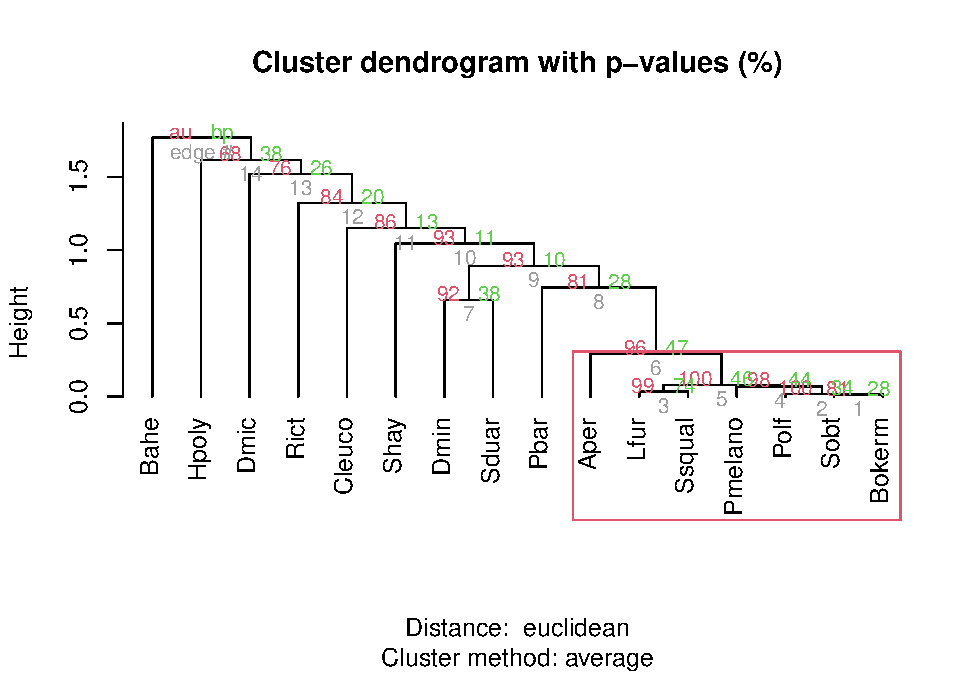
\includegraphics{livro_r_ecologia_files/figure-latex/unnamed-chunk-29-1.pdf}

\hypertarget{interpretauxe7uxe3o-dos-resultados-4}{%
\subsubsection{Interpretação dos resultados}\label{interpretauxe7uxe3o-dos-resultados-4}}

Com base no número de espécies raras, o estimador Jackknife 2 calculou a possibilidade de encontrarmos mais dez espécies caso o esforço amostral fosse maior e não mostrou tendência estabilização da curva em uma assíntota.

\hypertarget{bootstrap-smith-van-belle-1984}{%
\subsection{BOOTSTRAP (Smith \& van Belle 1984):}\label{bootstrap-smith-van-belle-1984}}

Este método difere dos demais por utilizar dados de todas as espécies coletadas para estimar a riqueza total, não se restringindo às espécies raras. Ele requer somente dados de incidência. A estimativa pelo bootstrap é calculada somando-se a riqueza observada à soma do inverso da proporção de amostras em que cada espécie ocorre.

\begin{quote}
\[S_{boot} = S_{obs} + \sum_{k=1}^{S_{obs}}(1-P_k)^m\]
\end{quote}

onde:

\begin{itemize}
\item
  Sobs = o número de espécies na comunidade,
\item
  \emph{m} = número de amostragens,
\item
  Pk = proporção do número de amostras em que cada espécie foi registrada.
\end{itemize}

~

\hypertarget{exemplo-pruxe1tico---bootstrap}{%
\subsubsection{Exemplo prático - Bootstrap}\label{exemplo-pruxe1tico---bootstrap}}

\hypertarget{explicauxe7uxe3o-dos-dados-5}{%
\paragraph{Explicação dos dados}\label{explicauxe7uxe3o-dos-dados-5}}

Usaremos os mesmos dados de 17 espécies de anuros amostradas em 14 dias de coletas de campo em um habitat reprodutivo localizado na região noroeste do estado de São Paulo, Brasil.

\textbf{Pergunta:}

\begin{quote}
Quantas espécies a mais poderiam ser amostradas caso aumentassemos o esforço amostral?
\end{quote}

\textbf{Predições}

\begin{quote}
\begin{itemize}
\tightlist
\item
  O número de espécies estimadas é similar ao número de espécies observada;
\item
  O número de espécies estimadas é maior do que o número de espécies observada.
\end{itemize}
\end{quote}

\textbf{Variáveis}

\begin{itemize}
\tightlist
\item
  Variáveis preditoras

  \begin{itemize}
  \tightlist
  \item
    matriz ou vetor com as abundâncias das espécies de anuros registradas em um habitat reprodutivo
  \end{itemize}
\end{itemize}

\textbf{Checklist}

\begin{itemize}
\tightlist
\item
  Verificar se a sua matriz está com as espécies nas colunas e as amostragens nas linhas
\end{itemize}

\hypertarget{anuxe1lise-5}{%
\subsection{Análise}\label{anuxe1lise-5}}

Calculo do estimador de riqueza - Bootstrap

\begin{Shaded}
\begin{Highlighting}[]
\KeywordTok{library}\NormalTok{(vegan)}
\NormalTok{dados_coleta <-}\StringTok{ }\NormalTok{poca_anuros}
\NormalTok{est_boot <-}\StringTok{ }\KeywordTok{poolaccum}\NormalTok{(dados_coleta, }\DataTypeTok{permutations =} \DecValTok{100}\NormalTok{)}
\KeywordTok{summary}\NormalTok{(est_boot, }\DataTypeTok{display =} \StringTok{"boot"}\NormalTok{)}
\end{Highlighting}
\end{Shaded}

\begin{verbatim}
## $boot
##        N Bootstrap      2.5%    97.5%  Std.Dev
##  [1,]  3  12.17185  8.329630 16.52037 2.310424
##  [2,]  4  13.12457  8.510840 17.41406 2.232225
##  [3,]  5  13.95024  9.841424 17.24064 1.967627
##  [4,]  6  14.53536 11.558721 18.22111 1.958557
##  [5,]  7  15.04432 11.829765 18.51122 1.878727
##  [6,]  8  15.73462 12.268670 19.62760 1.978622
##  [7,]  9  16.34148 12.613206 19.79883 1.887096
##  [8,] 10  16.93769 13.882703 19.59521 1.743707
##  [9,] 11  17.52273 13.890260 19.81162 1.673485
## [10,] 12  18.22123 15.233568 19.58724 1.410507
## [11,] 13  18.71802 16.570376 19.59107 1.035912
## [12,] 14  19.27832 19.278321 19.27832 0.000000
## 
## attr(,"class")
## [1] "summary.poolaccum"
\end{verbatim}

Visualizar os resultados com intervalo de confiança de 95\%

\begin{Shaded}
\begin{Highlighting}[]
\KeywordTok{library}\NormalTok{(ggplot2)}
\CommentTok{# preparando os dados para fazer o gráfico}
\NormalTok{resultados_boot <-}\StringTok{ }\KeywordTok{summary}\NormalTok{(est_boot, }\DataTypeTok{display =} \KeywordTok{c}\NormalTok{(}\StringTok{"S"}\NormalTok{, }\StringTok{"boot"}\NormalTok{))}
\NormalTok{res_boot <-}\StringTok{ }\KeywordTok{cbind}\NormalTok{(resultados_boot}\OperatorTok{$}\NormalTok{boot[,}\DecValTok{1}\OperatorTok{:}\DecValTok{4}\NormalTok{], resultados_boot}\OperatorTok{$}\NormalTok{S[,}\DecValTok{2}\OperatorTok{:}\DecValTok{4}\NormalTok{])}
\NormalTok{res_boot <-}\StringTok{ }\KeywordTok{as.data.frame}\NormalTok{(res_boot)}
\KeywordTok{colnames}\NormalTok{(res_boot) <-}\StringTok{ }\KeywordTok{c}\NormalTok{(}\StringTok{"Amostras"}\NormalTok{, }\StringTok{"BOOT"}\NormalTok{, }\StringTok{"BOOT_inferior"}\NormalTok{, }\StringTok{"BOOT_superior"}\NormalTok{, }\StringTok{"Riqueza"}\NormalTok{,}
                        \StringTok{"R_inferior"}\NormalTok{, }\StringTok{"R_superior"}\NormalTok{)}

\CommentTok{# comando para o gráfico}
\KeywordTok{ggplot}\NormalTok{(res_boot, }\KeywordTok{aes}\NormalTok{(}\DataTypeTok{y =}\NormalTok{ Riqueza, }\DataTypeTok{x =}\NormalTok{ Amostras)) }\OperatorTok{+}
\StringTok{  }\KeywordTok{geom_point}\NormalTok{(}\KeywordTok{aes}\NormalTok{(}\DataTypeTok{y =}\NormalTok{ BOOT, }\DataTypeTok{x =}\NormalTok{ Amostras }\OperatorTok{+}\StringTok{ }\FloatTok{0.1}\NormalTok{), }\DataTypeTok{size =} \DecValTok{5}\NormalTok{, }\DataTypeTok{color =} \StringTok{"blue"}\NormalTok{, }\DataTypeTok{alpha =} \DecValTok{1}\NormalTok{) }\OperatorTok{+}
\StringTok{  }\KeywordTok{geom_point}\NormalTok{(}\KeywordTok{aes}\NormalTok{(}\DataTypeTok{y =}\NormalTok{ Riqueza, }\DataTypeTok{x =}\NormalTok{ Amostras), }\DataTypeTok{size =} \DecValTok{5}\NormalTok{, }\DataTypeTok{color =} \StringTok{"red"}\NormalTok{, }\DataTypeTok{alpha =} \DecValTok{1}\NormalTok{) }\OperatorTok{+}
\StringTok{  }\KeywordTok{geom_line}\NormalTok{ (}\KeywordTok{aes}\NormalTok{(}\DataTypeTok{y =}\NormalTok{ BOOT, }\DataTypeTok{x =}\NormalTok{ Amostras), }\DataTypeTok{color =} \StringTok{"blue"}\NormalTok{) }\OperatorTok{+}
\StringTok{  }\KeywordTok{geom_line}\NormalTok{ (}\KeywordTok{aes}\NormalTok{(}\DataTypeTok{y =}\NormalTok{ Riqueza, }\DataTypeTok{x =}\NormalTok{ Amostras), }\DataTypeTok{color =} \StringTok{"red"}\NormalTok{) }\OperatorTok{+}
\StringTok{  }\KeywordTok{geom_linerange}\NormalTok{(}\KeywordTok{aes}\NormalTok{(}\DataTypeTok{ymin =}\NormalTok{ BOOT_inferior, }\DataTypeTok{ymax =}\NormalTok{ BOOT_superior, }\DataTypeTok{x =}\NormalTok{ Amostras }\OperatorTok{+}\StringTok{ }\FloatTok{0.1}\NormalTok{),}
 \DataTypeTok{color =} \StringTok{"blue"}\NormalTok{) }\OperatorTok{+}
\StringTok{  }\KeywordTok{geom_linerange}\NormalTok{(}\KeywordTok{aes}\NormalTok{(}\DataTypeTok{ymin =}\NormalTok{ R_inferior, }\DataTypeTok{ymax =}\NormalTok{ R_superior, }\DataTypeTok{x =}\NormalTok{ Amostras), }\DataTypeTok{color =} \StringTok{"red"}\NormalTok{) }\OperatorTok{+}
\StringTok{  }\KeywordTok{ylab}\NormalTok{ (}\StringTok{"Estimador de riqueza - Bootstrap"}\NormalTok{) }\OperatorTok{+}
\StringTok{  }\KeywordTok{xlab}\NormalTok{ (}\StringTok{"Número de amostras"}\NormalTok{) }\OperatorTok{+}
\StringTok{  }\KeywordTok{scale_x_continuous}\NormalTok{(}\DataTypeTok{limits =} \KeywordTok{c}\NormalTok{(}\DecValTok{1}\NormalTok{,}\DecValTok{15}\NormalTok{), }\DataTypeTok{breaks=}\KeywordTok{seq}\NormalTok{(}\DecValTok{1}\NormalTok{,}\DecValTok{15}\NormalTok{,}\DecValTok{1}\NormalTok{)) }\OperatorTok{+}
\StringTok{  }\KeywordTok{geom_point}\NormalTok{(}\DataTypeTok{y=} \FloatTok{10.4}\NormalTok{, }\DataTypeTok{x =} \FloatTok{9.5}\NormalTok{, }\DataTypeTok{size =} \DecValTok{5}\NormalTok{, }\DataTypeTok{color =} \StringTok{"blue"}\NormalTok{, }\DataTypeTok{alpha =} \DecValTok{1}\NormalTok{) }\OperatorTok{+}\StringTok{ }
\StringTok{  }\KeywordTok{geom_point}\NormalTok{(}\DataTypeTok{y=} \FloatTok{9.3}\NormalTok{, }\DataTypeTok{x =} \FloatTok{9.5}\NormalTok{, }\DataTypeTok{size =} \DecValTok{5}\NormalTok{, }\DataTypeTok{color =} \StringTok{"red"}\NormalTok{, }\DataTypeTok{alpha =} \DecValTok{1}\NormalTok{) }\OperatorTok{+}\StringTok{ }
\StringTok{  }\KeywordTok{geom_label}\NormalTok{( }\DataTypeTok{y =} \FloatTok{10.4}\NormalTok{, }\DataTypeTok{x =} \FloatTok{12.3}\NormalTok{, }\DataTypeTok{label =} \StringTok{"Riqueza estimada - Bootstrap"}\NormalTok{) }\OperatorTok{+}
\StringTok{  }\KeywordTok{geom_label}\NormalTok{( }\DataTypeTok{y =} \FloatTok{9.3}\NormalTok{, }\DataTypeTok{x =} \FloatTok{11.5}\NormalTok{, }\DataTypeTok{label =} \StringTok{"Riqueza observada"}\NormalTok{)}
\end{Highlighting}
\end{Shaded}

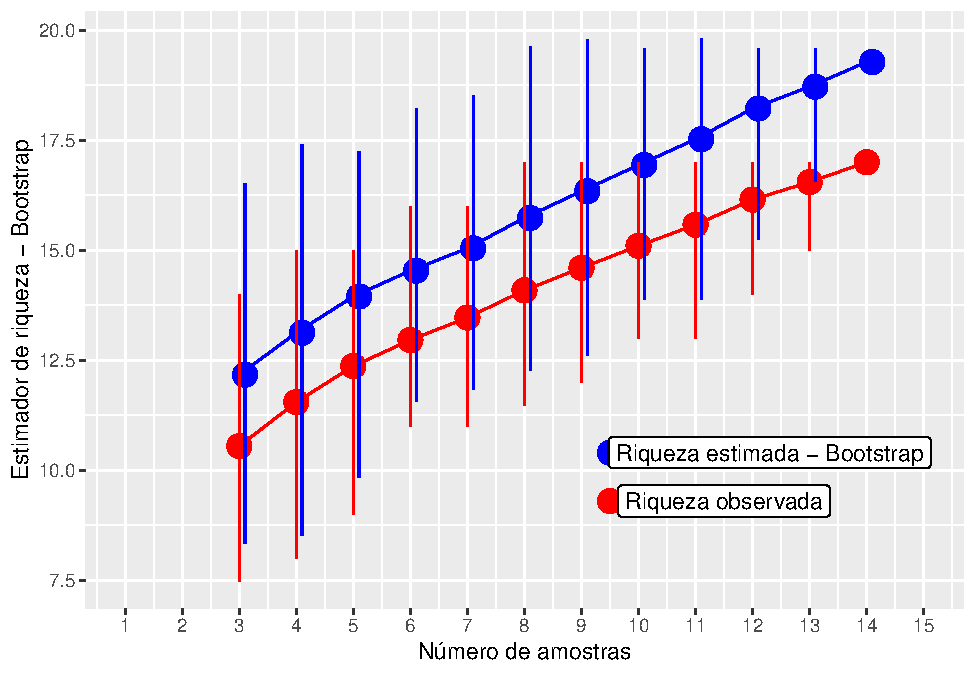
\includegraphics{livro_r_ecologia_files/figure-latex/unnamed-chunk-31-1.pdf}

\hypertarget{interpretauxe7uxe3o-dos-resultados-5}{%
\subsubsection{Interpretação dos resultados}\label{interpretauxe7uxe3o-dos-resultados-5}}

Com base na frequencia de ocorrência das espécies, o estimador bootstrap calculou a possibilidade de encontrarmos mais duas espécies caso o esforço amostral fosse maior e não mostrou tendência de estabilização da curva em uma assíntota.

\hypertarget{interpolauxe7uxe3o-e-extrapolauxe7uxe3o-baseadas-em-rarefauxe7uxe3o-usando-amostragens-de-inciduxeancia-ou-abunduxe2ncia-chao-jost-2012-colwell-et-al.-2012}{%
\subsection{Interpolação e Extrapolação baseadas em rarefação usando amostragens de incidência ou abundância (Chao \& Jost 2012, Colwell et al.~2012):}\label{interpolauxe7uxe3o-e-extrapolauxe7uxe3o-baseadas-em-rarefauxe7uxe3o-usando-amostragens-de-inciduxeancia-ou-abunduxe2ncia-chao-jost-2012-colwell-et-al.-2012}}

Este método utiliza teoria de amostragem (e.g.~modelos multinomial, Poisson e Bernoulli) para conectar rarefação (interpolação) e predição (extrapolação) com base no tamanho da amostra. Contudo, é importante enfatizar que a extrapolação torna-se altamente incerta quando extendida para o dobro do tamanho da amostragem. Este método utiliza uma abordagem com bootstrap para calcular o intervalo de confiança de 95\%. Uma das vantagens desta abordagem é que ela permite além da riqueza de espécies, interpolar e extrapolar os índices de diversidade de Shannon entropy (i.e.~quantifica a incerteza da identidade da espécie baseado na amostragem aleatória de um indivíduo da comunidade) e Gini-Simpson (i.e.~quantifica a probabilidade que dois indivíduos escolhidos aleatoriamente sejam de diferentes espécies). Contudo, estes índices de diversidades são transformados e apresentados em unidades de riqueza de espécies (\emph{Números de Hill}, Hill 1973). Hill percebeu que poderíamos calcular a riqueza de espécies máxima usando os índices de Shannon entropy e Gini-Simpson quando consideramos que todas as espécies na comunidade possuem abundâncias idênticas (máxima equitabilidade). Então, eles propos a transformação dos indíces de diversidade determinando qual seria o número de espécies equivalente da nossa comunidade (observado) se todas as espécies fossem igualmente abundantes (teórico). Desta maneira, os indíces podem ser comparavéis pois estão representados pela mesma unidade - riqueza de espécies. Os números de Hill são representados pelo parâmetro \emph{q} que controla a sensibilidide do índice em relação a abudância relativa das espécies (Gotelli \& Chao 2013). Quando q = 0 ele não considera a abundância das espécies e é igual a riqueza de espécies. Quando q = 1 ele é o exponencial da diversidade de Shannon, que dá uma peso maior para as espécies raras. Quando q = 2 ele é a diversidade de Simpson, que dá um peso maior para as espécies mais comuns na comunidade.

\hypertarget{exemplo-pruxe1tico}{%
\subsubsection{Exemplo prático}\label{exemplo-pruxe1tico}}

\hypertarget{explicauxe7uxe3o-dos-dados-6}{%
\paragraph{Explicação dos dados}\label{explicauxe7uxe3o-dos-dados-6}}

Usaremos os mesmos dados de 17 espécies de anuros amostradas em 14 dias de coletas de campo em um habitat reprodutivo localizado na região noroeste do estado de São Paulo, Brasil.

\textbf{Pergunta:}

\begin{quote}
Quantas espécies a mais poderiam ser amostradas caso aumentassemos o esforço amostral?
\end{quote}

\textbf{Predições}

\begin{quote}
\begin{itemize}
\tightlist
\item
  O número de espécies estimadas é similar ao número de espécies observada;
\item
  O número de espécies estimadas é maior do que o número de espécies observada.
\end{itemize}
\end{quote}

\textbf{Variáveis}

\begin{itemize}
\tightlist
\item
  Variáveis preditoras

  \begin{itemize}
  \tightlist
  \item
    matriz ou vetor com as abundâncias das espécies de anuros registradas em um habitat reprodutivo
  \end{itemize}
\end{itemize}

\textbf{Checklist}

\begin{itemize}
\tightlist
\item
  Verificar se a sua matriz está com as espécies nas colunas e as amostragens nas linhas.
\end{itemize}

\hypertarget{anuxe1lise-6}{%
\subsection{Análise}\label{anuxe1lise-6}}

Calculo da extrapolação da riqueza com base no número de indivíduos

\begin{Shaded}
\begin{Highlighting}[]
\KeywordTok{library}\NormalTok{(iNEXT)}
\NormalTok{dados_coleta <-}\StringTok{ }\NormalTok{poca_anuros}

\CommentTok{# preparando os dados para análises considerando a abundância}
\NormalTok{dados_inext_abu <-}\StringTok{ }\KeywordTok{colSums}\NormalTok{(dados_coleta) }

\NormalTok{resultados_abundancia <-}\StringTok{ }\KeywordTok{iNEXT}\NormalTok{(dados_inext_abu, }\DataTypeTok{q =} \DecValTok{0}\NormalTok{, }\DataTypeTok{datatype =} \StringTok{"abundance"}\NormalTok{, }
			\DataTypeTok{endpoint =} \DecValTok{600}\NormalTok{)}

\CommentTok{# Visualizar os dados no gráfico}
\KeywordTok{ggiNEXT}\NormalTok{(resultados_abundancia, }\DataTypeTok{type =} \DecValTok{1}\NormalTok{)}
\end{Highlighting}
\end{Shaded}

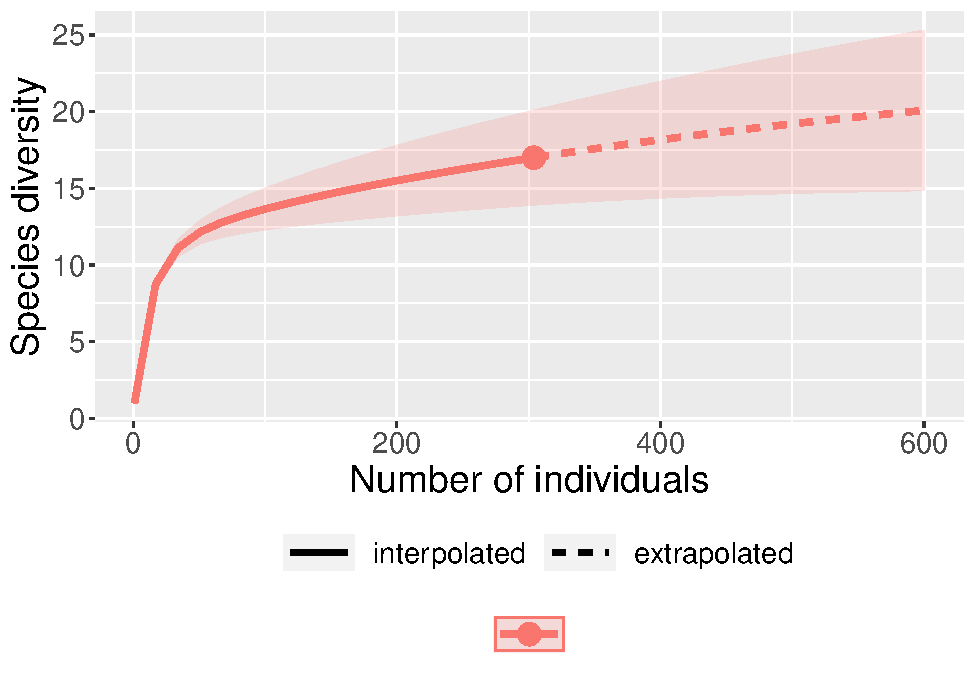
\includegraphics{livro_r_ecologia_files/figure-latex/unnamed-chunk-32-1.pdf}

\hypertarget{interpretauxe7uxe3o-dos-resultados-6}{%
\subsubsection{Interpretação dos resultados}\label{interpretauxe7uxe3o-dos-resultados-6}}

Veja que o ponto no final da linha contínua representa as 17 espécies de anuros (eixo Y) observadas entre os 304 individuos (eixo X). A extrapolação máxima (600 indivíduos no nosso exemplo), estima um aumento de até oito espécies (intervalo de confiança) caso amostrássemos mais 300 indivíduos.

Calculo da extrapolação da riqueza com base no número de amostras

\begin{Shaded}
\begin{Highlighting}[]
\KeywordTok{library}\NormalTok{(iNEXT)}
\NormalTok{dados_coleta <-}\StringTok{ }\NormalTok{poca_anuros}

\CommentTok{# preparando os dados para análises considerando a incidência}
\NormalTok{dados_inext <-}\StringTok{ }\KeywordTok{as.incfreq}\NormalTok{(}\KeywordTok{t}\NormalTok{(dados_coleta)) }\CommentTok{# preciso transpor o dataframe}

\NormalTok{resultados_incidencia <-}\StringTok{ }\KeywordTok{iNEXT}\NormalTok{(dados_inext, }\DataTypeTok{q =} \DecValTok{0}\NormalTok{, }\DataTypeTok{datatype =} \StringTok{"incidence_freq"}\NormalTok{, }
			\DataTypeTok{endpoint =} \DecValTok{30}\NormalTok{)}

\CommentTok{# Visualizar os dados no gráfico}
\KeywordTok{ggiNEXT}\NormalTok{(resultados_incidencia, }\DataTypeTok{type =} \DecValTok{1}\NormalTok{)}
\end{Highlighting}
\end{Shaded}

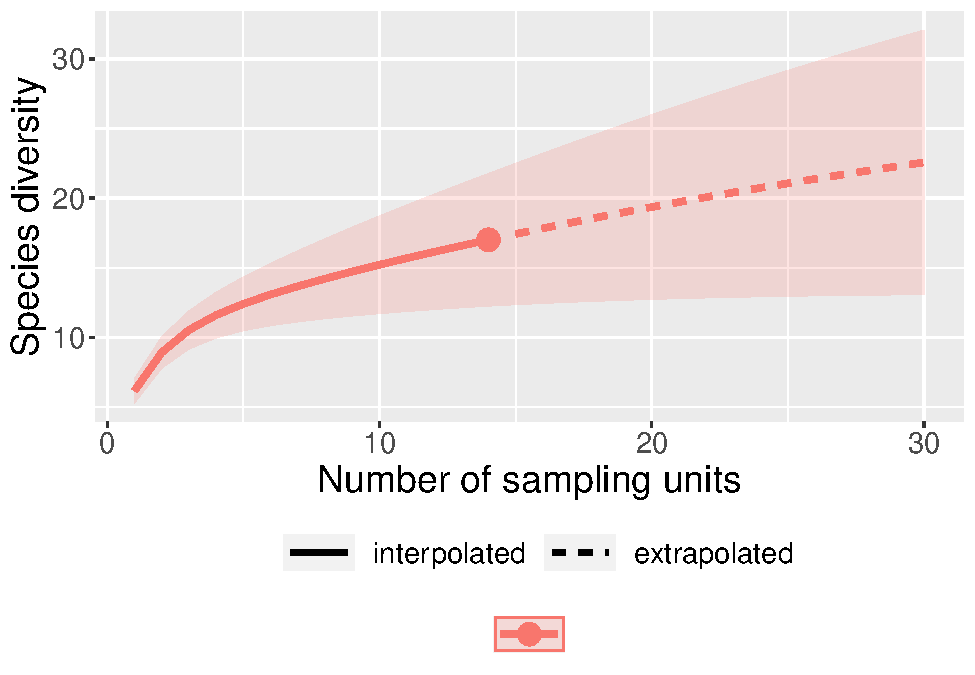
\includegraphics{livro_r_ecologia_files/figure-latex/unnamed-chunk-33-1.pdf}

\hypertarget{interpretauxe7uxe3o-dos-resultados-7}{%
\subsubsection{Interpretação dos resultados}\label{interpretauxe7uxe3o-dos-resultados-7}}

Veja que o ponto no final da linha contínua representa as 17 espécies de anuros (eixo Y) observadas nos 14 dias de coleta (eixo X - amostras). A extrapolação máxima (30 dias de coleta no nosso exemplo), estima um aumento de até 13 espécies (intervalo de confiança) caso amostrássemos mais 16 dias.

~

\hypertarget{para-se-aprofundar}{%
\subsection{Para se aprofundar}\label{para-se-aprofundar}}

\begin{itemize}
\item
  Recomendamos aos interessados que olhem a página do \href{http://viceroy.eeb.uconn.edu/estimates}{EstimateS software} e baixem o manual do usuário que contém informações detalhadas sobre os índices de rarefação e estimadores de riqueza.Este site foi criado e é mantido pelo Dr.~Robert K. Colwell, um dos maiores especialistas do mundo em estimativas da biodiversidade
\item
  Recomendamos também o livro Magurran \& McGill (2010) - Biological Diversity Frontiers in Measurement and Assessment.
\end{itemize}

  \bibliography{book.bib,packages.bib}

\end{document}
